\chapter{Image views}
\label{chap:image_views}

\lettrine[lines=2]{T}{his} concept of views is not new~\parencite{novak.1997.reuse} and naturally appeared in Image
processing with Milena under the name of \emph{morpher}~\parencite{levillain.2009.ismm, geraud.2012.hdr}. It was always
useful to be able to project an image through a prism that could extract specific information about it without the need
to copy the underlying data buffer. In modern days, the language C++ (20) also introduces this mechanism with the
ranges~\parencite{niebler.2014.ranges} facilities for \emph{non-owning collections}. It is named \emph{views} and allows
the user to access the content of a container (vector, map) through a prism. In Pylene, we decided to align the naming
system after what was decided in C++20 in order not to confuse the user. This way, a \texttt{transform} view in image
processing will do the same thing on an image that the transform view in the standard range library does on a container.
\emph{Views} feature the following properties: \emph{cheap to copy}, \emph{non-owner} (does not \emph{own} any data
buffer), \emph{lazy evaluation} (accessing the value of a pixel may require computations) and \emph{composition}. When
chained, the compiler builds a \emph{tree of expressions} (or \emph{expression template} as used in many scientific
computing libraries such as Eigen~\parencite{guennebaud.2010.eigen}), thus it knows at compile-time the type of the
composition and ensures a 0-overhead at evaluation. We will first motivate the usage of \emph{views} in image
processing. We will then present the main views used in image processing. Then will be discussed how image views differ
from the one used in C++'s ranges and their main properties (especially how they keep/discard the properties from the
parent image) through a concrete example: the management of border and extension policies. Finally, we will discuss the
limitations of such a design.

\section{The Genesis of a new abstraction layers: Views}
\label{sec:genesis_of_views}

In image processing an algorithm is naively written by taking one or several inputs' data (among which is the input
image(s)),  by performing work on this input data and then by returning the resulting data (or an error). Let us take
for example the alpha-blending example which can be implemented in naive C++ code as followed:
\begin{minted}{C++}
  void blend_inplace(const uint8_t* ima1, uint8_t* ima2, float alpha,
  int width, int height, int stride1, int stride2) {
    for (int y = 0; y < height; ++y) {
      const uint8_t* iptr = ima1 + y * stride1;
      uint8_t* optr = ima2 + y * stride2;
      for (int x = 0; x < width; ++x)
        optr[x] = iptr[x] * alpha + optr[x] * (1-alpha);
    }
  }
\end{minted}

This code has several flaws. It makes strong hypothesis about the input images: its data buffer contiguity and its shape
(2D). Let us suppose that our user now wants to restrict the algorithm to a specific region inside the image. The
maintainer would have then to provide an overload of the algorithm with one additional input argument corresponding to the
region of interest. Let us suppose that the user now wants to support manipulate 3D images. The maintainer would now
have to provide two additional overloads with an additional stride argument (one for the base algorithm, one for the
region of interest-restricted algorithm). Let us now suppose that the user only wants to manipulate the red color
channel. Now the maintainer must support and additional overloads of the algorithm for each channel and/or color type.
The complexity increases manyfold for each kind of customization points the maintainer wants to offer to the user. Of
course, it is possible to prevent code duplication through clever usage of computer engineering techniques (code
factorization etc.) but the complexity would still leak through the API anyway. That is way the other solution is to
make the user able to perform those restriction upstream from the algorithm transparently so that the downstream
algorithm is easy to write, understand and maintain. In order to achieve this, we need to raise the abstraction level
around images by one layer so that we can work at the image level. The alpha-blending algorithm would then be written as
shown in~\cref{fig:view.alphablend}.

\begin{figure}[htbp]
  \centering
  \includestandalone[mode=image, scale=0.7]{../figures/alphablend}

  \caption{Alpha-blending algorithm written at image level.}
  \label{fig:view.alphablend}
\end{figure}

This way to express an algorithm is achieved by introducing \emph{views} to image processing. An image now is a view and
can be restricted/projected/manipulated however the user need before feeding it to an algorithm. Even the whole alpha
blending algorithm can be rewritten in terms of views entirely, as shown in~\cref{fig:new.alphablend}.

\begin{figure}[htbp]
  \centering
  \begin{minipage}[b]{5.5cm}
    \includestandalone[mode=image, scale=1.0]{../figures/view_ast2}
  \end{minipage}
  \begin{minipage}[b]{5.5cm}
    \begin{minted}{c++}
    auto alphablend =
      [](auto ima1, auto ima2, float alpha) {
        return alpha * ima1 + (1 - alpha) * ima2;
      };
    \end{minted}
    \bigskip
    \bigskip
    \bigskip
  \end{minipage}
  \caption{Alpha-blending, generic implementation with \emph{views}, expression tree.}
  \label{fig:new.alphablend}
\end{figure}

Being able to perform powerful manipulation on images before feeding them to algorithms completely nullify the initial
problem of having several overloads of the same algorithm while maintaining and documenting all the associated optional
arguments. Indeed, in order to perform the alpha-blending transformation on the base input image, all that the user must
do is:
\begin{minted}{C++}
  auto ima1, ima2 = /* ... */;
  auto ima_blended = alphablend(ima1, ima2, 0.2);
\end{minted}
If the user wants to restrict the region to be blended, or the color channel to work on, he just has to write the
following modification:
\begin{minted}{C++}
  auto roi = /* ... */;
  auto blended_roi = alphablend(view::clip(ima1, roi), view::clip(ima2, roi), 0.2);
  auto blended_red = alphablend(view::red(ima1), view::red(ima2), 0.2);
\end{minted}
The restriction is done upstream from the algorithm and propagated downstream without increasing the code complexity.
This way, view greatly increase what the user can do by writing less code.

\section{Views for image processing}
\label{sec:viws_for_ip}

There are four fundamental kinds of views, inspired by functional programming paradigm: \texttt{transform(input, f)}
applies the transformation \(f\) on each pixel of the image \emph{input},\\
\texttt{filter(input, pred)} keeps the pixels of \emph{input} that satisfy the predicate \emph{pred},
\texttt{clip(input, domain)} keeps the pixels of \emph{input} that are in the \emph{domain}, \texttt{zip(\(input_1\),
  \(input_2\), \ldots, \(input_n\))} allows to pack several pixels of several images to iterate on them all at the same
time. From those four fundamentals come out more very useful views such as \texttt{cast<T>(input)} or
\texttt{mask(input, msk)} that are more specific to the image processing area.

In Pylena, the practitioner can use a large array of views. Those views come into different form and allow the
practitioner to seamlessly use arithmetic or logic operators on images like he would when using expression template. We
separate the available views in two main families: the views that perform a restriction of the domain (clip, filter) and
the views that transform the values (transform, zip).

\subsection{Domain-restricting views}

\paragraph{The filter view} It is also a fundamental view which consists in keeping only the values that satisfy a
predicate. This is very useful when working with thresholds as shown in the following code:
\begin{minted}{C++}
auto my_threshold = 145;
auto inferior_to [my_threshold](uint8_t val) { return val <= my_threshold; };
auto superiorstrict_to = [](uint8_t val) { return not inferior_to(val); };
mln::image2d<uint8_t> ima_grayscale = /* ... */;
auto ima_inferior = mln::view::filter(ima_grayscale, inferior_to);
auto ima_superiorstrict = mln::view::filter(ima_grayscale, superiorstrict_to);
mln::fill(ima_inferior, 0u8);
mln::fill(ima_superiorstrict, 255u8);
\end{minted}
This code shows a way to binarize \texttt{ima\_grayscale} with a custom threshold using the filter view. It is important
to note that the resulting filtered image has its domain of definition changed. And the new domain of definition will
most likely not be in a regular usual shape (such as a 2D rectangle). This implies that the usage of this view inside
certain algorithms may be limited.

\paragraph{The clip view} It is a convenient way to extract a sub-image from a base image. This view essentially
redefine the domain of definition to restrict it into a smaller one. It does not change anything else which means it
proxies every access to the image. For instance, we make use of this view to easily subdivide a 2D-image into 4 tiles as
shown in the code below:
\begin{minted}{C++}
  mln::image2d<mln::rgb8> large_image = /* ... */;
  point2d shape = large_image.domain().shape();
  auto middle_pnt = point2d{shape.x() / 2, shape.y() / 2};
  auto tl = large_image.domain().tl(); // top-left point
  auto br = large_image.domain().br(); // bottom-right point
  auto four_tiles = std::tuple{
    mln::view::clip(ima, mln::box2d{tl, middle_pnt}),   // top-left tile
    mln::view::clip(ima, mln::box2d{                    // top-right tile
      point2d{middle_pnt.x(), tl.y()},
      point2d{br.x(), middle_pnt.y()}
      }),
    mln::view::clip(ima, mln::box2d{                    // bottom-left tile
      point2d{tl.x(), middle_point.y()},
      point2d{middle_pnt.x(), br.y()}
    }),
    mln::view::clip(ima, mln::box2d{middle_pnt, br})   // bottom-right tile
  };
\end{minted}

\paragraph{The mask view} It is very image-processing oriented as it allows the practitioner to provide a boolean image
the same size as the original image to select only the pixels whose corresponding value in the mask is true. Its usage
is shown in the following code:
\begin{minted}{C++}
  mln::image2d<mln::rgb8> ima = /* ... */;
  auto mask = ima > 127;
  mln::fill(mln::view::mask(ima, mask), 255);
\end{minted}
This code set all the values that are superior to 127 to the max value 255. It shows that it can both be used with read
and write access.


\subsection{Value-transforming views}

\paragraph{The transform view} It is the most important view of all. It consists in applying a function to each image's
pixel. For instance, writing the grayscale algorithm with a transform view is as simple as the following code:
\begin{minted}{C++}
  auto grayscale_transform = [](mln::rgb8 val) -> uint8_t {
    return 0.2126 * v[0]    // red
           + 0.7152 * v[0]  // green
           + 0.0722 * v[0]; // blue
  };
  mln::image2d<mln::rgb8> ima_rgb = /* ... */;
  mln::image2d<uint8_t>   ima_grayscale = mln::view::transform(ima_rgb, grayscale_transform);
\end{minted}
There is no loop in this code, just the pixel-wise transformation function. Furthermore, the code will not compute the
resulting image. The computation will happen on-the-fly each time a value from \texttt{ima\_grayscale} is yielded.
This view allows the practitioner to quickly write and adapt any pixel-wise algorithm he needs for his more complex
calculation efficiently.

\paragraph{The zip view} It is one of the most useful view and allow the practitioner to iterate over a set of image at
the same time. The basic use-case consists in iterating over a set of input image and the output image to be able to
consistently assign output values to a resulting computation from input values. Its usage is shown in the following
code:
\begin{minted}{C++}
  mln::image2d<uint8_t> input = /* ... */;
  mln::image2d<uint8_t> output{input.domain()};
  auto zipped_ima = mln::view::zip(input, output);
  for (auto&& [v_in, v_out] : zipped_ima.values())
    v_out = v_in < 145 ? 0 : 255; // binarisation
\end{minted}
This code is another example of how to compute a binary threshold image.

\paragraph{The channel/RGB views} It is a projector to access a specific color channel of an image. There exists image
with many more channels than just the standard red/green/blue ones, from the astrophysics or medical area for instances.
This view is a tool to restrict an image and only access a specific channel. Its usage is shown in the following code:
\begin{minted}{C++}
  mln::image2d<mln::rgb8> ima = /* ... */;
  mln::copy(mln::view::red(ima), mln::view::green(ima));
\end{minted}
This code copies the red component into the green component. It shows that the view can be used in both read and write
access. Another more generic view exists; \mintinline{c++}{mln::view::channel(ima, k)}, that access the \texttt{k}-th
channel in \texttt{ima}.

\paragraph{The cast views} It is a way to convert an image's underlying type to another type, by performing a cast. As
this does not modify the underlying value in itself, the access cannot be a write access. This view can be used as shown
in
the following code:
\begin{minted}{C++}
  mln::image2d<double> ima = /* ... */;
  mln::image2d<uint8_t> ima_8bits = mln::view::cast<uint8_t>(ima);
\end{minted}

\paragraph{The arithmetical operators} \(+, -, *, /, \%\) are implemented in the form of transformation views that
operate point-wise between two images whose size is identical. For instance, writing the following code:
\begin{minted}{C++}
  mln::image2d<uint8_t> ima1 = /* ... */;
  mln::image2d<uint8_t> ima2 = /* ... */;
  auto ret = ima1 + ima2;
\end{minted}
Is equivalent to writing the following code:
\begin{minted}{C++}
  auto ret = mln::view:transform(ima1, ima2, [](auto v1, auto v2){ return v1 + v2; });
\end{minted}
It is important to note that the \texttt{-} unary operator is also supported: \mintinline{C++}{-ima1}.

\paragraph{The logical operators} \(<, <=, ==, !=, >, >=\) are implemented in the same way that arithmetical operators
are. Both unary and binary operators are expressed as transform views such as writing the following code:
\begin{minted}{C++}
  auto ret = !ima1 && ima2;
\end{minted}
is equivalent to writing the following code:
\begin{minted}{C++}
  auto tmp = mln::view::transform(ima1, [](auto v){ return !v; });
  auto ret = mln::view::transform(tmp, ima2, [](auto v1, auto v2){ return v1 && v2; });
\end{minted}
It is far more expressive and more comprehensible by the practitioner. Also, a new facility is introduced to express the
logic behind a ternary expression (if C then A else B): the operator \(ifelse(C, A, B)\). The rationale is to be able to
swap between values depending on a boolean mask. This way, a mathematical morphology algorithm such as \emph{hit or
  miss} can be implemented in the following simple manner:
\begin{minted}{C++}
  mln::image2d<uint8_t> ima = /* ... */;
  auto ero = erode(ima);
  auto dil = dilate(ima);
  uint8_t zero = 0;
  auto ret = mln::view::ifelse(dil < ero, ero - dil, zero);
\end{minted}
Everything is taken care of and the practitioner just has to write down his algorithm to get it done.

\paragraph{The mathematical operators} They are implemented in the form of views that operates point-wise. The supported
mathematical operators are the following: abs, pow, sqr, cbrt, sqrt, sum, prod, min, max, dot, cross, l0norm, l1norm,
l2norm, l2norm\_sqr, linfnorm, lpnorm, l0dist, l1dist, l2dist, l2dist\_sqr, linfdist, lpdist. Calling an operator onto
an image is equivalent to calling a transform view on each value of this image:
\begin{minted}{C++}
  auto ima = /* ... */;
  auto ret = view::maths::abs(ima);
\end{minted}
Is equivalent to calling:
\begin{minted}{C++}
  auto ima = /* ... */;
  auto ret = view::transform(ima, [](auto v){ return std::abs(v); });
\end{minted}


\section{View properties}
\label{sec:views_properties}

Views feature interesting properties, especially how they keep/discard the properties of the concrete image they are
based on. However, before talking about those properties, it is important to draw the line and point the main
differences between the C++20 ranges views and our image views.

\subsection{Differences between C++20 ranges views and image views}
\label{subsec:C++20_views_vs_image_views}

C++20 ranges views are a new abstraction layer introduced on top of the already existing iterators. This means that a
view is created from an existing container from its iterators. There are also special views such as
\texttt{std::views::iota} that are able to generate an infinite sequence of number. Those last are the generator views
and are designed to be used the same way as a container, except that they do not own any data. In C++20 the views are
mainly constructed from a container such as \texttt{std::vector}, \texttt{std::map} or \texttt{std::list}. For instance,
the way to create a view featuring all the elements of a container is shown in the following code:
\begin{minted}{C++}
  auto vec = std::vector { /* ... */ };
  auto vec_vw = std::views::all(vec);
\end{minted}
This induces issues regarding dangling references when passing temporary views or when the container owning the data
expires. To summarize the model of ranges in C++20, they are a new abstraction layer much more friendly and powerful
than iterators and can construct non-owning, cheap-to-copy views from an owning container.

\subsection{Data ownership}

The concept of \emph{View} brought to us a fundamental issue when dealing with images: \blockquote{\emph{What is an
    image?}}. More precisely: should an image always be the owner of its data buffer? Should we have a shared ownership of
the data buffer between all the images using it? Then what happens when the data changes? The issue about the semantic
of an image is crucial but also very similar to the issue there is to differentiate a \emph{container} (such as
\texttt{std::vector}, that is to say the data buffer) and a \emph{view}, as seen
in~\cref{subsec:C++20_views_vs_image_views}.

From here we have considered two approaches. The first one is to have \emph{shared ownership} of the data buffer for the
image and its derived views. However, this does not allow the differentiation between an already computed image and a
lazy image. To be able to make this differentiation is crucial in an \emph{Image Processing library} as we want to make
the most out of the data we already have, and we do not want to compute data we do not need. Also, we cannot distinguish
when the \emph{copyability} property is required. This is the main reason why we did not adopt this approach.

The second one is to make the differentiation between a \emph{concrete image} which owns the data (like the standard
containers) and the \emph{views} that are lightweight cheap-to-copy objects. However, this would imply we have to
distinguish both image families when writing algorithms, and we do not want that.

This is why we have chosen to take a path where we mix both approaches at the same time. We assert that all image are
cheap-to-copy (including views), even the concrete images. The concrete image will have a shared ownership semantic
related to its data buffer and will remain cheap-to-copy. It will also behave the same way a view behaves. That is why,
with our semantic, all images are views. Ultimately, there is still a way to distinguish a view from a concrete image,
if needed, and we introduce two new concepts \texttt{ViewImage} and \texttt{ConcreteImage} for this end:
\begin{minted}{C++}
template <typename I>
concept ConcreteImage =
  Image<I> &&
  std::concepts::semiregular<I> &&  // A concrete image is default constructible
  not image_view_v<I>;

template <typename I>
concept ViewImage =
  Image<I> &&
  image_view_v<I>;
\end{minted}
Having images as views is a very important property as it simplify greatly the reasoning when performance is needed.
This allows the user to pass his images everywhere without worrying about dangling data buffer expiring around the
corner. It also enables us to have a library design similar to the C++'s standard library which the user is familiar
with and, why not, have standard algorithm and standard view work on our image types. All of these are the main reason
why we decided to adopt this design. However, unlike the standard library, as we are not required to work with iterator
due to backward compatibility.

\begin{figure}[htbp]
  \centering
  \begin{minipage}{\linewidth}
    \includestandalone[mode=image, width=.7\linewidth]{../figures/transform_thresholding}
  \end{minipage}
  \caption{An image \emph{view} performing a thresholding.}
  \label{fig:view.threshold}
\end{figure}

In our design, all images are lightweight (cheap-to-copy) objects with shared ownership over the data. A view image is a
non-owning image that only stores pointers, as shown in~\cref{fig:view.threshold}. A concrete image stores the data. The
only difference between a view and a concrete image is given by a trait \texttt{image\_view} which will check the
\texttt{view} property of the given image to tell whether it is a concrete owning image type or not. Compared to the
C++20 ranges views model, mechanism prevent errors resulting from dangling references and confusing ownership of data.
It is especially adapted to image processing as the user generally wants to avoid deep copy of its data. When the user
wants to deep-copy his image (clone) he wants to do it explicitly.

This design induces one major property which is the \emph{lazy-evaluation} of the views.

\subsection{Lazy evaluation, composability and chaining}
\label{subsec:image.views.lazy.eval}

The key point of views is the lazy evaluation. When a concrete image is piped through a view, no computation is done.
The computation happens when the practitioner requests a value by doing \(val = V(p)\). The implications are multiples:
an image can be piped into several computation-heavy views, some of which can be discarded later on, and it will not
impact the performance. Also, when processing large images, applying a transformation on a part of the image (such as
clipping or filtering) is as simple as restricting the domain with a view and applying the transformation to this
resulting sub-image.

\emph{Lazy-evaluation} combined with the view \emph{chaining} allows the user to write clear and very efficient code
whose evaluation is delayed till very last moment as shown in~\cref{fig:lazy} (see \parencite{geraud.2018.gtgdmm} for
additional examples). Neither memory allocation nor computation are performed; the image \(i\) has just recorded all the
operations required to compute its values.

\begin{figure}[htbp]
  \begin{minipage}[l]{0.48\linewidth}
    \begin{minted}{C++}
image2d<rgb8>  ima1 = /* ... */;
image2d<uint8_t> ima2 = /* ... */;

// Projection: project the red channel value
auto f = view::transform(ima1, [](auto v) {
  return v.r;
});

// Lazy-evaluation of the element-wise
// minimum
auto g = view::transform(view::zip(f, ima2),
  [](auto value) {
    return std::min(std::get<0>(value),
             std::get<1>(value));
});
\end{minted}
  \end{minipage}
  \hfill
  \begin{minipage}[l]{0.48\linewidth}
    \begin{minted}{C++}
// Lazy-Filtering: keep pixels whose value
// is below < 128
auto h = view::filter(g, [] (auto value) {
  return value < 128;
}));

// Lazy-evaluation of a gamma correction
using value_t = typename Image::value_type;
constexpr float gamma = 2.2f;
constexpr auto max_val =
  std::numeric_limits<value_t>::max();
auto i = view::transform(h,
  [gamma_corr = 1 / gamma, max_val] (auto value) {
    return std::pow(value / max_val,
             gamma_corr) * max_val;
});
\end{minted}
  \end{minipage}

  \caption{Lazy-evaluation and \emph{view} chaining.}
  \label{fig:lazy}
\end{figure}

The tree of type resulting from this view chaining is illustrated by~\cref{fig:viewAST}. It illustrates how chaining
views with each other result in the formation of an abstract tree that records the operations to perform. This model
enables building complex computational trees via views while keeping efficient performance at runtime. However, those
trees are complex for the compiler to process and can induce heavy compilation time overhead.

\begin{figure}[htb]
  \centering
  \includegraphics[width=8cm]{../figures/viewAST2}
  \caption{Abstract Syntax Tree of the types chained by the code in~\cref{fig:lazy}}
  \label{fig:viewAST}
\end{figure}


\subsection{Preserving image properties}

Views will also try to preserve properties of the original image when they can. That means that views can preserve the
ability of the practitioner to, for instance, write into this image. This may be a trivial property to preserve when
considering a view that restrict a domain, but when considering a view that transforms the resulting values, it is not.
Let us consider the projection \(h: (r,g,b) \mapsto g\) that selects the green component of an RGB triplet. When piping
the resulting view into, for instance, a blurring algorithm, the computation will take be performed in place thanks to
the fact we still have the ability to write into the image. A legacy way of obtaining the same result would have been to
create a temporary single-channel image to extract the green channel of the original RGB image so that the temporary
image could then be blurred. The final step would have then been to copy the values of the temporary blurred image back
into the green channel of the original image. The comparison, including the memory used, between the legacy way and the
in-place way of doing this computation is shown in~\cref{fig:legacy.vs.view}.

\begin{figure}[htbp]
  \centering
  \subfloat[Legacy pipeline with copy]{
    \includegraphics[width=1.6in,align=t]{../figures/blur_copy}
  }
  \hfil
  \subfloat[Modern pipeline with view]{
    \includegraphics[width=1.6in,align=t]{../figures/blur_inplace}
  }

  \caption{Comparison of a legacy and a modern pipeline using \emph{algorithms} (green) and \emph{views} (purple).}
  \label{fig:legacy.vs.view}
\end{figure}

On the other hand, when considering the view \(g: (r,g,b) \mapsto 0.2126*r+0.7152*g+0.0722*b\) that compute the gray
level of a color triplet (as shown in~\cref{fig:view.grayscale}), the ability to write a value into the image cannot be
preserved. Indeed, one would need an inverse function that is able to deduce the original color triplet from the gray
level to be able to write back into the original image. This operation alone is a whole field of research on its
own~\parencite{zhang.2016.colorful,levin.2004.colorization,welsh.2002.transferring}

\begin{figure}[htbp]
  \centering
  \includegraphics[width=.7\linewidth]{../figures/views/transform_grayscale}
  \caption{Usage of transform view: grayscale.}
  \label{fig:view.grayscale}
\end{figure}

\begin{figure}[htbp]
  \centering
  \subfloat[Clip view]{
    \includegraphics[width=3in,align=t]{../figures/clip}
  }
  \hfil
  \subfloat[Filter view]{
    \includegraphics[width=3in,align=t]{../figures/filter}
  }

  \caption{Clip and filter image adaptors that restrict the image domain by a non-regular ROI and by a predicate that
    selects only even pixels.}
  \label{fig:view.clip}
\end{figure}

Similarly, a view can apply a restriction on an image domain. In~\cref{fig:view.clip}, we show the adaptor
\texttt{clip(input, roi)} that restricts the image to a non-regular \texttt{roi} and \texttt{filter(input, predicate)}
that restricts the domain based on a predicate. All subsequent operations on those images will only affect the selected
pixels. In this case of restriction, the ability to write data back into the original image is preserved through the
view.

\begin{figure}[htbp]
  \centering
  \includegraphics[scale=0.7]{../figures/pipeline}
  \caption{Example of a simple image processing pipeline.}
  \label{fig:view.pipeline}
\end{figure}

Views feature many interesting properties that change the way we program an image processing application. To illustrate
those features, let us consider the following image processing pipeline: (Start) Load an input RGB-8 2D image (a
classical HDR photography) (A) Convert it in grayscale (B) Sub-quantize to 8-bits (C) Perform the grayscale dilation of
the image (End) Save the resulting 2D 8-bits grayscale image; as described in~\cref{fig:view.pipeline}. This pipeline is
expressed with two notions. The first notion is composition of \colorbox{lightgreen}{algorithms} (\(A \rightarrow B
\rightarrow C\)) in order to achieve the desired result. The second notion is the composition of
\colorbox{thistle}{views} (\(Input \rightarrow A \rightarrow B\)) which overlaps partially with the algorithm part. This
express that part of the algorithm is performed lazily only when we perform the last part (C). Those two notions are
illustrated by the~\cref{fig:view.comp}.

\begin{figure}[htbp]
  \centering
  \includegraphics[scale=0.7]{../figures/composition}
  \caption{Example of a simple image processing pipeline illustrating the difference between the composition of
    algorithms and image views.}
  \label{fig:view.comp}
\end{figure}

There are six properties one want to keep track when working with views: \emph{forward}, \emph{writable},
\emph{accessible}, \emph{indexable}, \emph{bidirectional} and \emph{raw}. Those properties echo to the concepts seen
in~\cref{sec:library.concepts}. An image is \emph{forward} when it can be traversed in a forward way. It is
\emph{writable} when the values are mutable. It is \emph{accessible} whenever it allows to access the value associated
to a point (\ie it allows to write the expression \(v = ima(p)\)). It is \emph{indexable} whenever its values can be
accessed through an index localizer (\ie it allows to write the expression \(v = ima[idx]\)). Usually, accessing
through an index is faster than accessing by a point. It is \emph{bidirectional} when it can be traversed in both a
forward and a backward way. Finally, an image is \emph{raw} when its data buffer can is contiguous and can directly be
accessed with information about strides. The~\cref{table:views.properties} presents all the views and how they preserve
the base properties of a concrete image.

\begin{table}[htbp]
  \begin{scriptsize}
    \begin{threeparttable}
      \caption{Views: property conservation}
      \begin{tabular}{|l|l|cccccc|}
        \hline
        \thead{View type}    & \diagbox{\thead{Expression}}{\thead{Property}} & Forward & Bidirectional & Raw    & Writable     & Accessible & Indexable \\
        %\thead{View type}    & \thead{Expression | Properties:} & Forward & Bidirectional & Raw    & Writable   & Accessible & Indexable \\
        \hline
        \thead{Image}        & \texttt{ima1, ima2}                            & \cmark  & \cmark        & \cmark & \cmark       & \cmark     & \cmark    \\
        \thead{Cast}         & \texttt{cast<T>(ima)}                          & \cmark  & \cmark        & \xmark & \xmark       & \cmark     & \cmark    \\
        \thead{Transform}    & \texttt{transform(ima, func)}                  & \cmark  & \cmark        & \xmark & \cmark\(^1\) & \cmark     & \cmark    \\
        \thead{Filter}       & \texttt{filter(ima, pred)}                     & \cmark  & \cmark        & \xmark & \xmark       & \cmark     & \cmark    \\
        \thead{Clip}         & \texttt{clip(ima, dom)}                        & \cmark  & \cmark        & \xmark & \cmark       & \cmark     & \cmark    \\
        \thead{mask}         & \texttt{mask(ima, mask)}                       & \cmark  & \cmark        & \xmark & \cmark       & \cmark     & \cmark    \\
        \thead{Zip}          & \texttt{zip(ima1, ima2)}                       & \cmark  & \cmark        & \xmark & \cmark       & \cmark     & \cmark    \\
        \thead{Channel}      & \texttt{red(ima)}                              & \cmark  & \cmark        & \xmark & \cmark       & \cmark     & \cmark    \\
        \thead{Arithmetic}   & \texttt{ima1 + ima2}                           & \cmark  & \cmark        & \xmark & \xmark       & \cmark     & \cmark    \\
        \thead{Logical}      & \texttt{ima > 125}                             & \cmark  & \cmark        & \xmark & \xmark\(^2\) & \cmark     & \cmark    \\
        \thead{Mathematical} & \texttt{abs(ima)}                              & \cmark  & \cmark        & \xmark & \xmark       & \cmark     & \cmark    \\
        \hline
      \end{tabular}
      \begin{tablenotes}
        \item \(^1\): writability is preserved only if \texttt{func} is a projection.
        \item \(^2\): writability not preserved except for the expression \texttt{ifelse(ima, ima1, ima2)}.
      \end{tablenotes}
      \label{table:views.properties}
    \end{threeparttable}
  \end{scriptsize}
\end{table}

Also, we may want to extend the property preservation discussion to other concepts we saw in the
previous~\cref{chap:image.algorithms.taxonomy}, especially the concepts of structuring element and extension.

\section{Decorating images to ease border management}
\label{sec:border.management}

When looking at local algorithms, we notice that a long recurring issue is about the behavior on the border of the
image. There are many ways of dealing with this problem. One is to allocate additional memory for the border and paste
values in it. Another is to check the bounds when looping over the neighbors inside the computational window. We can
also decorate the image to return a correct lazily computed value when accessing out-of-image-bound value still inside
the extension. The point is: all these methods have advantages as well as disadvantages.

\paragraph{Memory allocated border}
The border width is fixed at the image's creation and cannot be augmented without doing a reallocation. There is also a
cost when computing border's values (to fill it) which is proportional to the border's width and to the image's size. On
the other hand, the access time of a border value during the algorithm unrolling is as fast as a native access time
within the image itself. The last issue remaining would be that the border is not infinite. We cannot process a local
algorithm with a structuring element that does not fit in the extension. This method is especially adapted when there is
medium structuring elements with a known size which will yield a lot of out-of-image's bound accesses. When speed is
required, this method is a de facto standard.

\paragraph{Bound checking}
Assuming there is no border, and we are not allowed to access out-of-image-bound values, a bound check is required when
accessing each values. Another way to do would be to decorate the facility that yields the neighbors of a pixel: do not
yield out-of-image-bound pixels. This removes the need to bound check for each pixel's value which is relatively
faster. The caveats of this method are that it induces a slight slow down when yielding the pixel's neighbors from the
structuring element, and that it is not always viable: some algorithms do need to access values in an extension to
produce proper results.

\paragraph{Image decoration}
The border is infinite, and we make a view of our image to decorate it with the required extension. This is achieved
using \emph{views}: the original image is chained into a view that will add the required feature to the image. For
instance, let us consider the following image:
\begin{minted}{C++}
struct borderless_image {
  // ...
  // NO extension_type subtype
  // NO extension() method
};
\end{minted}

Attempting to use this image in a local algorithm that works with a structuring element as the structuring element does
not fit inside the image when considering the behavior on the borders. However, instead of narrowing the region of
interest, it is possible to make a view that will return an image from which the behavior at the border is well-defined.
Referring to the taxonomy from the previous~\cref{chap:image.algorithms.taxonomy} we remember that we can construct a
custom extension type for the sake of an example (as described in~\cref{subsec:local.se.ext}). This example will
decorate the image so that the border is always filled with a specific value. The following code shows how we can write
such an extension:
\begin{minted}{C++}
template <class ValueType>
struct FillExt {
  using support_fill = std::true_type; // Support the fill policy
  bool is_fill_supported() const { return true; }

  using value_type = ValueType;        // Underlying value_type

  // Always fit structuring element of any size
  template <class StructuringElement>
  bool fit(const StructuringElement& se) const { return true; }

  void fill(ValueType v) { v_ = v; }  // Assign the filled value
  // ...
  // Yield the value for a given point (always return filled value)
  template <class PointType>
  ValueType val(PointType) const { return v_; }
  // ...
  private:
    ValueType v_;
};
\end{minted}

Now that our extension type is written, we introduce a new image type which will adapt our base
\texttt{borderless\_image} into a view which features out \texttt{FillExt} extension type.
\begin{minted}{C++}
template <class BaseImage>
struct filled_border_image : image_view_adaptor<BaseImage>{
  // ...
  using extension_type = FillExt;
  extension_type& extention() const { ext_; }
  // ...

  value_type at(point_type pnt) {
    if(!domain().has(pnt)) {
      return extension().val()
    }
  }
  // ... adapt all the methods that can make out-of-bound access and fallback on
  // the extension's value ...
private:
  extension_type ext_;
};
\end{minted}

Finally, all that is left to do is to write the function that will construct the view from the base image:
\begin{minted}{C++}
template <class BaseImage>
auto fill_extension_view(BaseImage ima) {
  // call to the image_view_adaptor ctor
  auto with_fill_ext_ima = filled_border_image<BaseImage>(ima);
  return with_fill_ext_ima; // <-- this is a view
}
\end{minted}

This simple function enables very powerful usage as illustrated in the code below:
\begin{minted}{C++}
  auto ima = image2d<uint8_t>{
    {0, 1, 2},
    {3, 4, 5}
    {6, 7, 8}
  };
  ima.at({1, 1}); // OK, 4
  ima.at({5, 5}); // ERROR, out-of-bound
  // Get a view
  auto ima_with_filled_border = fill_extension_view(ima);
  // Fill border with value 255
  ima_with_filled_border.extension().fill(255);
  ima_with_filled_border.at({5, 5}); // OK, 255
\end{minted}

For the sake of brevity we have simplified the implementation in our example. In practice the implementation of such a
pattern is more complex as there are many strategies to support, the interfaces of the extension may be different, the
decoration of the image type may not be enough, notably for the \emph{none} strategy where it is required to decorate
the structuring element.

At the end, this method has the advantage to \textit{always work}. Given any structuring element of any size, any
algorithm will work. The disadvantage is that we need to check for out-of-bound access at the image level, and lazily
compute the value in case of out-of-image-bound access. The slowness induced is not negligible and should be weighted
carefully.

It is important to note the very close relation between an image's domain (to perform out-of-bound checks), the
structuring element (notably its size) and the extension (its width). A user may require, for a specific set of those
three elements, to decorate the image, and/or the structuring element and/or to perform computation and/or reallocation.
To resolve this issue, we decided to provide the user with a new facility: the \emph{border manager} whose job is to
prepare a suitable pair (image and structuring element) given a set of configuration wanted by the user.

We designed the configuration to be constructed from a given set of a policy and a method. We currently offer two
policies: native and auto.

\begin{itemize}
  \item Native: if the border is large enough: forward the image as-is to the algorithm to allow the fastest access
        possible. Otherwise, the border manager fails and halt the program.
  \item Auto: if the border is large enough: forward the image as-is to the algorithm to allow the fastest access
        possible. Otherwise, decorate the image with a view whose extension will emulate what is required by the
        algorithm with the given structuring element.
\end{itemize}

We also provide seven different methods to fill up our extension with the wanted values. It is important to note that
not all the methods are available for both policies. The policies are: none, fill, mirror, periodize, clamp, image and
user.

The \emph{none} policy enforces a policy where there is no border to use. The method cannot fail as it enforces the
border to vanish. To enforce this method, the border manager decorates the structuring element in a view that checks the
domain inclusion of each neighboring point. The \emph{fill} policy enforces that the border is filled with a specific
value. The \emph{mirror} policy enforces that the border is filled with a mirrored value from an axial symmetry relative
to the image's edges. The \emph{periodize} policy enforces that the border replicate the image, like a mosaic. The
\emph{clamp} policy enforces that the border is filled with values expanded from the values at the image's edge. The
\emph{image} policy enforces all points out of the current image's domain are to be picked inside another image. A basic
use-case is preparing tiles from a large image. The position of our image can be offset in the image acting as an
extension which ease the usage when, for instance, clipping a sub-image. The~\cref{fig:border.all} shows how a sub-image
(tile) can consider the base image as its border. Finally, the \emph{user} policy assumes the user knows what he is
doing and do not touch nor decorate the given image in any way. Both policies lead to the same behavior: check whether
the structuring element fit and then forward the image as-is if it fits. An exception is raised if it does not.
The~\cref{fig:border.all} illustrates all the other border policy mentioned.

\begin{figure}[htbp]
  \centering
  \subfloat[Border \emph{None}]{
    \includegraphics[width=1.8in,align=t]{../figures/extensions/none}
  }
  \hfil
  \subfloat[Border \emph{fill} w/ $0$]{
    \includegraphics[width=1.8in,align=t]{../figures/extensions/fill}
  }
  \hfil
  \subfloat[Border \emph{mirror}]{
    \includegraphics[width=1.8in,align=t]{../figures/extensions/mirror}
  }
  \hfil
  \subfloat[Border \emph{periodize}]{
    \includegraphics[width=1.8in,align=t]{../figures/extensions/periodize}
  }
  \hfil
  \subfloat[Border \emph{clamp}]{
    \includegraphics[width=1.8in,align=t]{../figures/extensions/clamp}
  }
  \hfil
  \subfloat[Border \emph{image}]{
    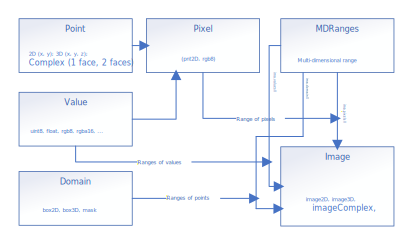
\includegraphics[width=1.8in,align=t]{../figures/extensions/image}
  }

  \caption{Border methods' breakdown.}
  \label{fig:border.all}
\end{figure}

As a consequence the usage of a local algorithm becomes very simple:

\begin{minted}{C++}
// default border width is 3
image2d<int> ima = {{0, 1, 0}, {0, 1, 1}, {0, 1, 0}};
auto disc_se = se::disc{1}; // radius is 1
auto bm = extension::bm::fill(0); // fill border with 0 with policy auto

local_algorithm(ima, disc_se, bm); // will handle the border for you
\end{minted}

The border manager \texttt{bm} is set with the method fill (with value 0) and policy \texttt{auto} (which is the default
policy). To use the policy \texttt{native}, one would write \texttt{extension::bm::native::fill(0)} instead.

In the implementation of the local algorithm, a dispatch is made with the pattern \emph{visitor}, relying on the
standard facilities \texttt{std::visit} and \texttt{std::variant} so that the performance overhead as well as the
complexity of use remain minimal. Let us assume we have a local algorithm implemented this way:
\begin{minted}{C++}
template <class Ima, class SE>
local_algorithm(Ima ima, SE se)
{
  // assume ima has a large enough border for the given se
  // use ima & se in loop
}
\end{minted}
We can rewrite it leveraging the border manager facility this way:
\begin{minted}{C++}
template <class Ima, class SE, class BM>
local_algorithm(Ima ima, SE se, BM bm)
{
  auto [managed_ima, managed_se] = bm.manage(ima, se);
  std::visit([&](auto&& ima_, auto&& se_) {
    // use ima_ & se_ in loop
    }, managed_ima, managed_se);
}
\end{minted}
The overhead is kept minimal thanks to using \texttt{std::variant} and \texttt{std::visit} and the algorithm implementer
delegate the border management to the border manager. This is made possible thanks to the views. Indeed, under the hood
the border manager may pipe the original image into a view that will behave accordingly to the policy chosen by the
user. This will be transparent from both practitioner and maintainer points of views.


\section{Views limitations}

Views can be of tremendous use in our area however it relies on metaprogramming techniques which are infamous for
greatly increasing the compilation time of source code. Also, when one starts to chain views a lot, combining different
image type (via \emph{zip} for instance), combined with the overhead induced via the border manager using
\texttt{std::variant}, the compilation time can really become an issue. Indeed, C++ developers tend to minimize the cost
of compilation time because once the program is compiled, the binaries can be distributed and are really fast to
execute. However, we are not exactly in that case as our library is generic. That means we distribute source code to our
user and our user compiles it when prototyping their program. This is an issue every library developer faces:
distributing heavily templated source code as a library can be a deal-breaker. In the industry, it was even to the point
that people refused to use boost in their code line. The boost maintainers had to modularize their library, so that user
is able to cherry-pick the parts he needs without pulling half of the library which was a disaster for the compile time
of a project.

The ranges for C++20's standard library and its views face the same issue. It was not rare for someone to need 90sec to
compile the calendar toy example of the library which just contains code that displays a given month in the classic
printed format (day number-of-month correctly displayed in column corresponding to the day of week label). This massive
compile time is due to early compiler implementation needing massive RAM usage for template type and having to swap when
the computer running the compilation was out of RAM. Now compilers have optimized the whole process, but the combination
behind the types can still be an issue. Introducing complex view code in a program that is compiled often may not be a
good idea. However, a program that is rarely compiled but is run a great number of time may take advantages of all the
optimizations the compiler do to be efficient.

\subsection{Image traversing with ranges}
\label{subsec.range.traversing}

Lastly, views usage should be measured when used at critical points. We learned from experience that one simple change
can make the compiler miss optimization opportunities which can greatly impact the resulting performance. Let us
illustrate our remark with a concrete example: image traversing. In previous version of our library, we used macro for
image traversing. \texttt{mln\_concrete}, \texttt{mln\_piter}, \texttt{mln\_qiter}, \texttt{for\_all} and
\texttt{mln\_value} are all macros aiming at hiding the underlying complexity. Our goal were to replace those macros
with existing C++ core language code to improve the user experience as well as ease the maintenance, contribution and
further improvement of the library. To do so, we based our image traversing on \texttt{std::ranges}. Let us take the old
implementation we had of our dilation algorithm as an example:
\begin{minted}{c++}
  template<class I, class SE>
  mln_concrete(I) dilate(const I& f, const SE& se)
  {
    mln_concrete(I) g;
    initialize(g, f);
    mln_piter(I) p(f.domain());
    mln_qiter(SE) q(se, p);
    for_all(p) // for all p in f domain
    {
      mln_value(I) v = f(p);
      for_all(q) // for all q in se(p)
        if(f.has(q) and f(q) > v)
          v = f(q);
      g(p) = v;
    }
    return g;
  }
\end{minted}

This code features the macro mentioned above and, while being explicit, may be quite obscure with regard to its
internals for a non-initiated user. However, it uses a double loop to traverse the image under the hood. Rewriting the
algorithm using ranges results in the following code:
\begin{minted}{c++}
  template<class I, , class SE>
  auto dilate(I input, const SE& se)
  {
    auto output = input.concretize(); // clone image
    for(auto [in_px, out_px] : view::zip(f.pixels(), g.pixels()))
    {
      out_px.val() = out_px.val();
      for(auto nhx : se(in_px))
        out_pix.val() = std::max(nhx.val(), out_px.val());
    }
    return output;
  }
\end{minted}
This code use the \emph{zip} view to iterate over two images (the input image and the resulting output image)
simultaneously. This is native code, and it should, in theory, be efficient than the old version of the code (with
macros) as it enables compiler optimizations such as vectorization or inner loops unrolling. But through benchmarking,
we have learned that this solution does not mix well~\parencite{austern.2000.segmented} with the multidimensional nature
of images. The issue originates from the fact that we have no way to explicitly say in the code that the
multidimensional range is made of chunk of contiguous rows of memory. Indeed, for each element we have to compute an
index originating from potentially \(N\) dimensions. This disables critical optimizations such as vectorization. We
solved this problem by augmenting range-v3's ranges with our own multidimensional ranges. Indeed, we only need to have
contiguity on the last dimension to provide the compiler code it can optimize. Which means that each for-loop that
traverses the whole n-dimensional image can be transformed into a double for-loop whose inner loop is guaranteed to be a
contiguous row. This way we have now an outer range as well as an inner range, as illustrated
in~\cref{fig:inner.outer.range}.

\begin{figure}[htbp]
  \centering
  \subcaptionbox{}{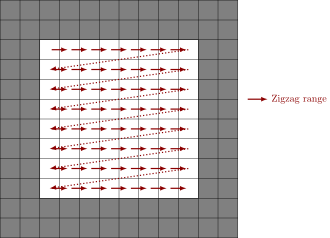
\includegraphics[width=.48\linewidth]{../figures/linear_rng}}
  \subcaptionbox{}{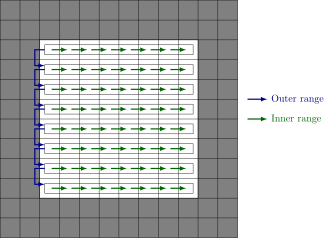
\includegraphics[width=.48\linewidth]{../figures/segmented_rng}}
  \caption{Range-v3's ranges (a) \vs multidimensional ranges (b).}
  \label{fig:inner.outer.range}
\end{figure}

Thanks to this new design we can now rewrite our algorithm with a double for-loop for the image traversing. Hopefully it
stays really similar to what one would be used to when working with the classical two-dimensional image. As an example,
we can rewrite the dilation algorithm this way:
\begin{minted}{c++}
template<class I, class SE>
auto dilate(I input, const SE& se)
{
  auto output = input.concretize(); // clone image
  // this line is needed to avoid dangling reference
  auto zipped_pixels = view::zip(input.pixels(), output.pixels());
  for(auto&& row : ranges::rows(zipped_pixels)) // unroll the contiguous segments
    for(auto [in_px, out_px] : row)             // optimized traversing of the segment
    {
      out_px.val() = out_px.val();
      for(auto nhx : se(in_px))
        out_pix.val() = std::max(in_px.val(), out_px.val());
    }
  return output;
}
\end{minted}

The highlight of this code is the usage a new tool: \texttt{ranges::rows} to bring out an inner range (contiguous) from
the multidimensional outer range.

\subsection{Performance discussion}

In order to have a relevant discussion on performance, we decided to implement a real world image processing pipeline:
the background subtraction. It is used to detect changes in image sequences~\parencite{opencv.bg_sub}. It is mainly used
when regions of interest are foreground objects. The pipeline components include: subtraction, Gaussian filtering,
threshold, erode and dilate, as shown in~\cref{fig:view.comp.sub_bg}.

\begin{figure}[htbp]
  \centering
  \includegraphics[width=0.7\linewidth]{../figures/pipeline_bg_sub_comp}
  \caption{Background subtraction pipeline using \colorbox{lightgreen}{algorithms} and
    \colorbox{thistle}{views}.}
  \label{fig:view.comp.sub_bg}
\end{figure}

The first thing that we notice is that the implementation of the pipeline using views is transcribed very explicitly in
the code, as shown in~\cref{fig:view.comp.sub_bg.view_code}. There is a direct correspondence between the graphic
pipeline and the code.

\begin{figure}
  \begin{minted}[highlightlines={3-4,6,8},highlightcolor=thistle]{c++}
  float kThreshold = 150; float kVSigma = 10;
  float kHSigma = 10;  int kOpeningRadius = 32;
  auto img_gray = view::transform(img_color, to_gray);
  auto bg_gray  = view::transform(bg_color, to_gray);
  auto bg_blurred = gaussian2d(bg_gray,  kHSigma, kVSigma);
  auto tmp_gray = img_gray - bg_blurred;
  auto thresholdf = [](auto x) { return x < kThreshold; };
  auto tmp_bin = view::transform(tmp_gray, thresholdf);
  auto ero = erosion(tmp_bin, disc(kOpeningRadius));
  dilation(ero, disc(kOpeningRadius), output);
  \end{minted}
  \caption{Pipeline implementation with \colorbox{thistle}{\emph{views}}. Highlighted code uses \emph{views} by
    prefixing operators with the namespace \texttt{view}.}
  \label{fig:view.comp.sub_bg.view_code}
\end{figure}

For our benchmark, we have decided to run the algorithm on an original set of image to detect a changing foreground.
We have considered 10 data set. We present in~\cref{fig:bg_sub.dataset_samples} three of them for the sake of brevity.

\begin{figure}[htbp]
  \centering
  \begin{tabular}{cccc}
    Background
                                                                                       & Candidate & Result                    \\[5pt]
    \fbox{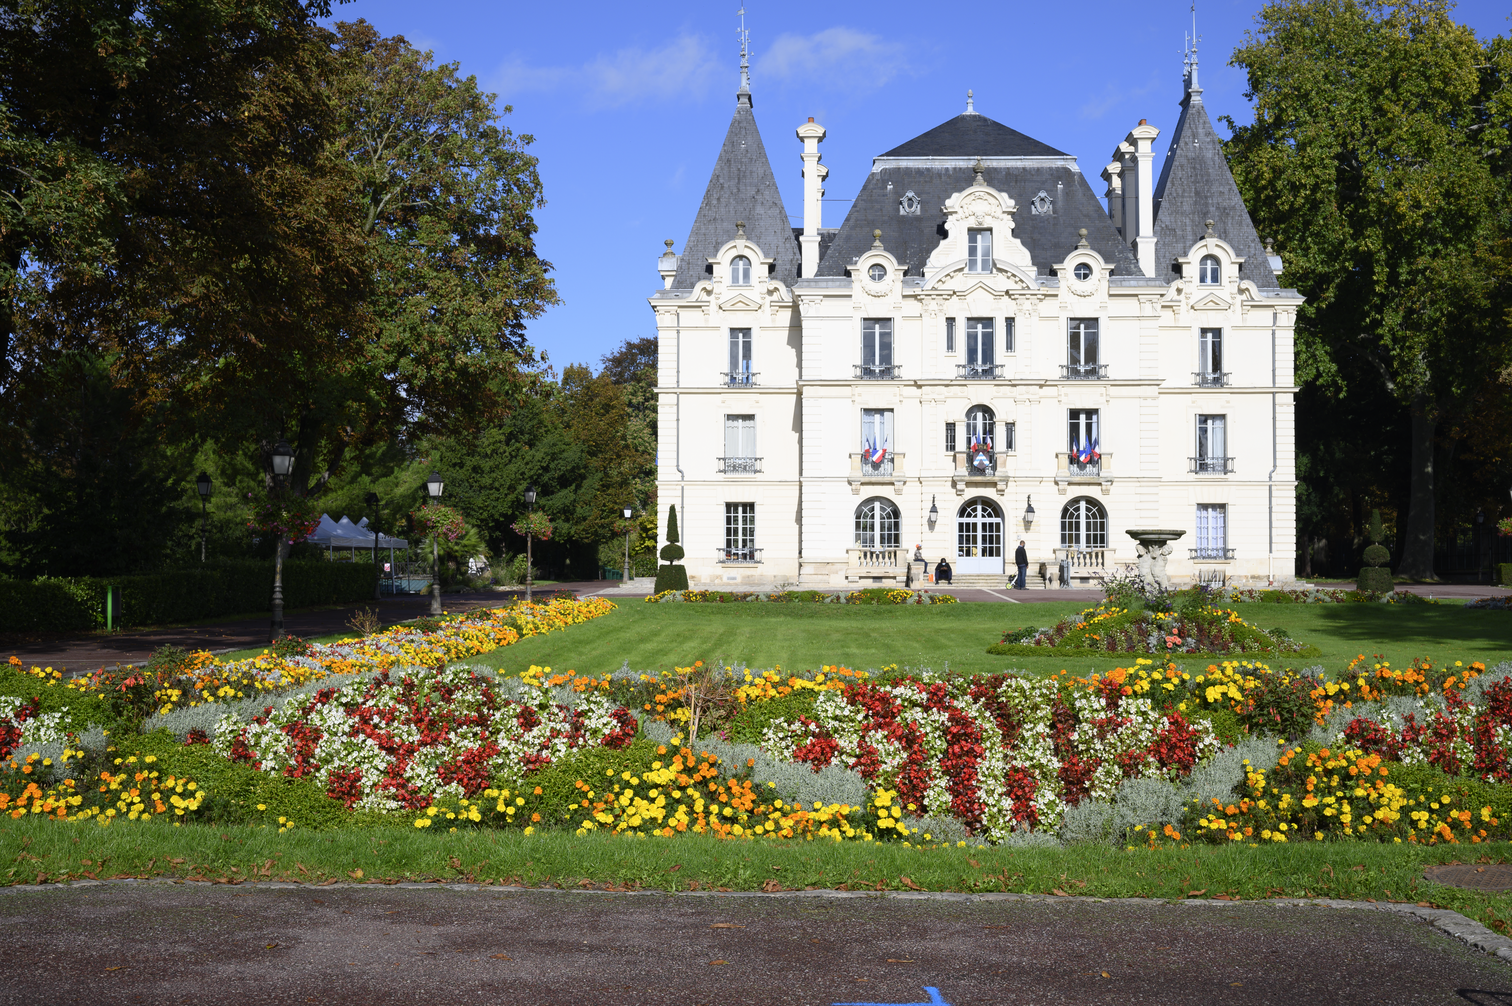
\includegraphics[width=.29\linewidth]{../assets/1512x1006/castle_bg.png}}    &
    \fbox{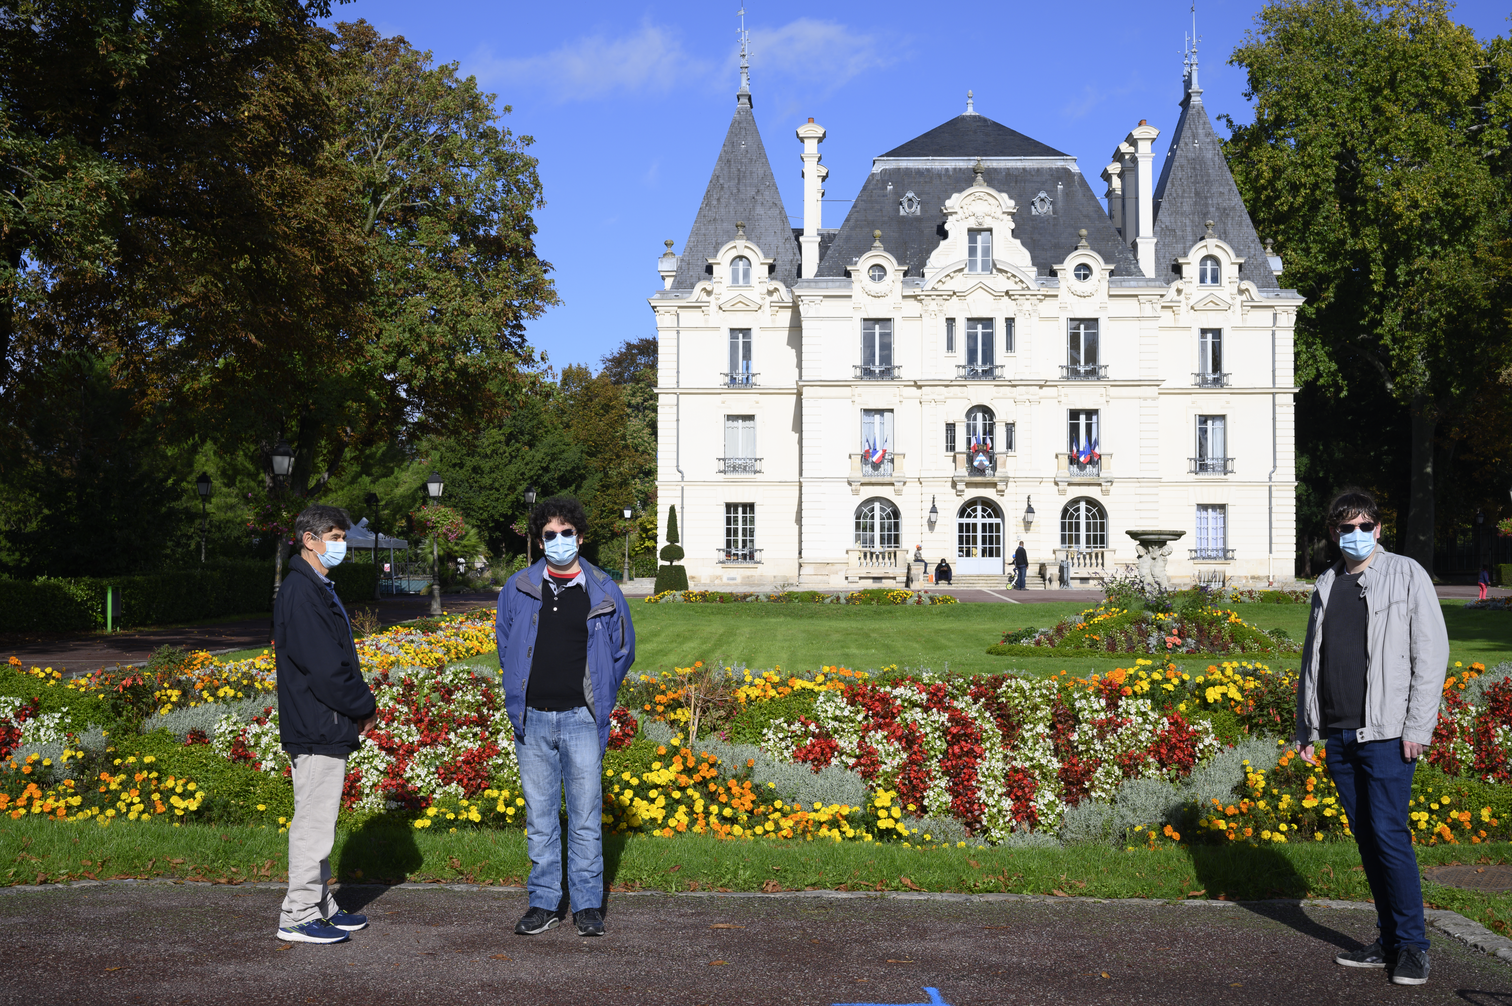
\includegraphics[width=.29\linewidth]{../assets/1512x1006/castle_fg_1.png}}  &
    \fbox{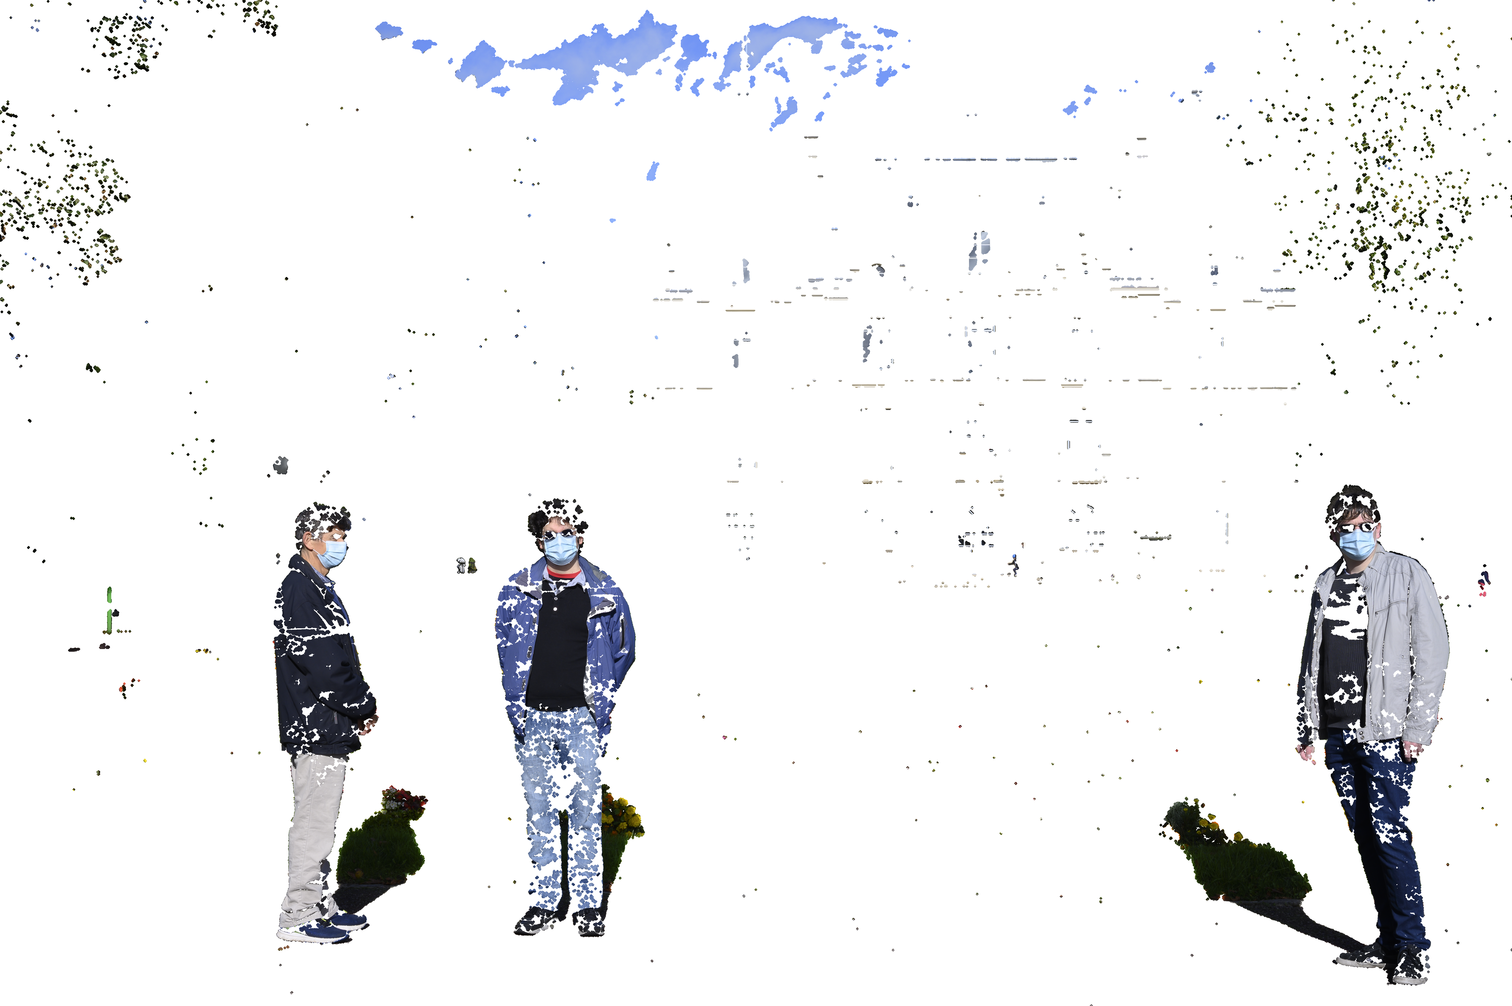
\includegraphics[width=.29\linewidth]{../assets/1512x1006/results_sig1_win5/castle/result_detected_castle_fg_1.png}} \\[5pt]
    \fbox{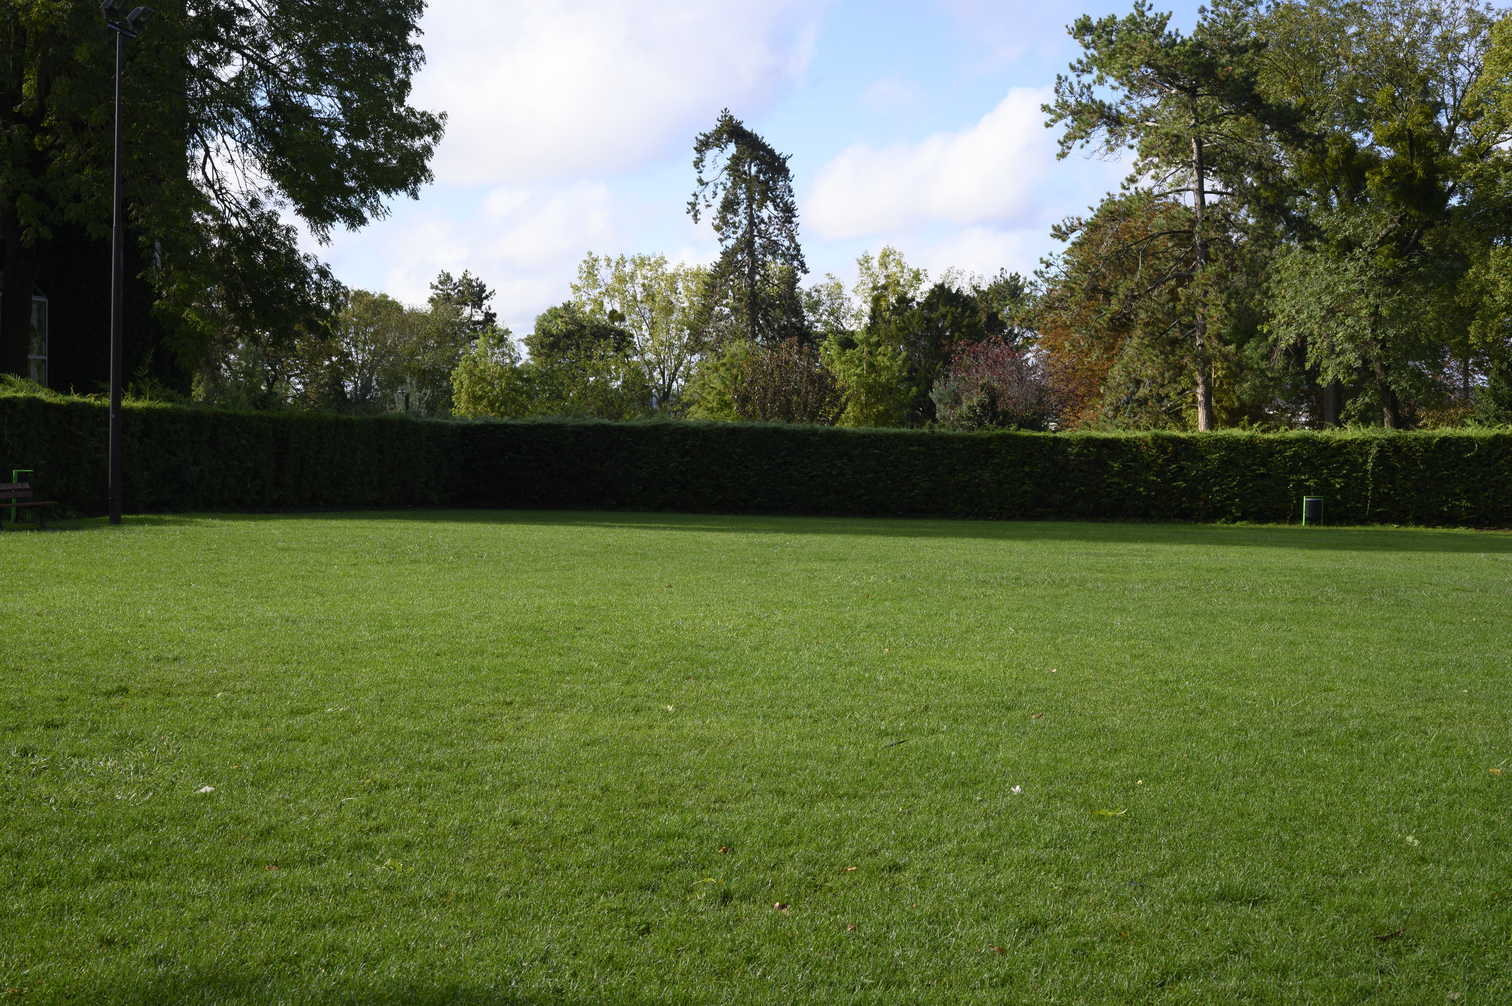
\includegraphics[width=.29\linewidth]{../assets/1512x1006/garden_bg.png}}    &
    \fbox{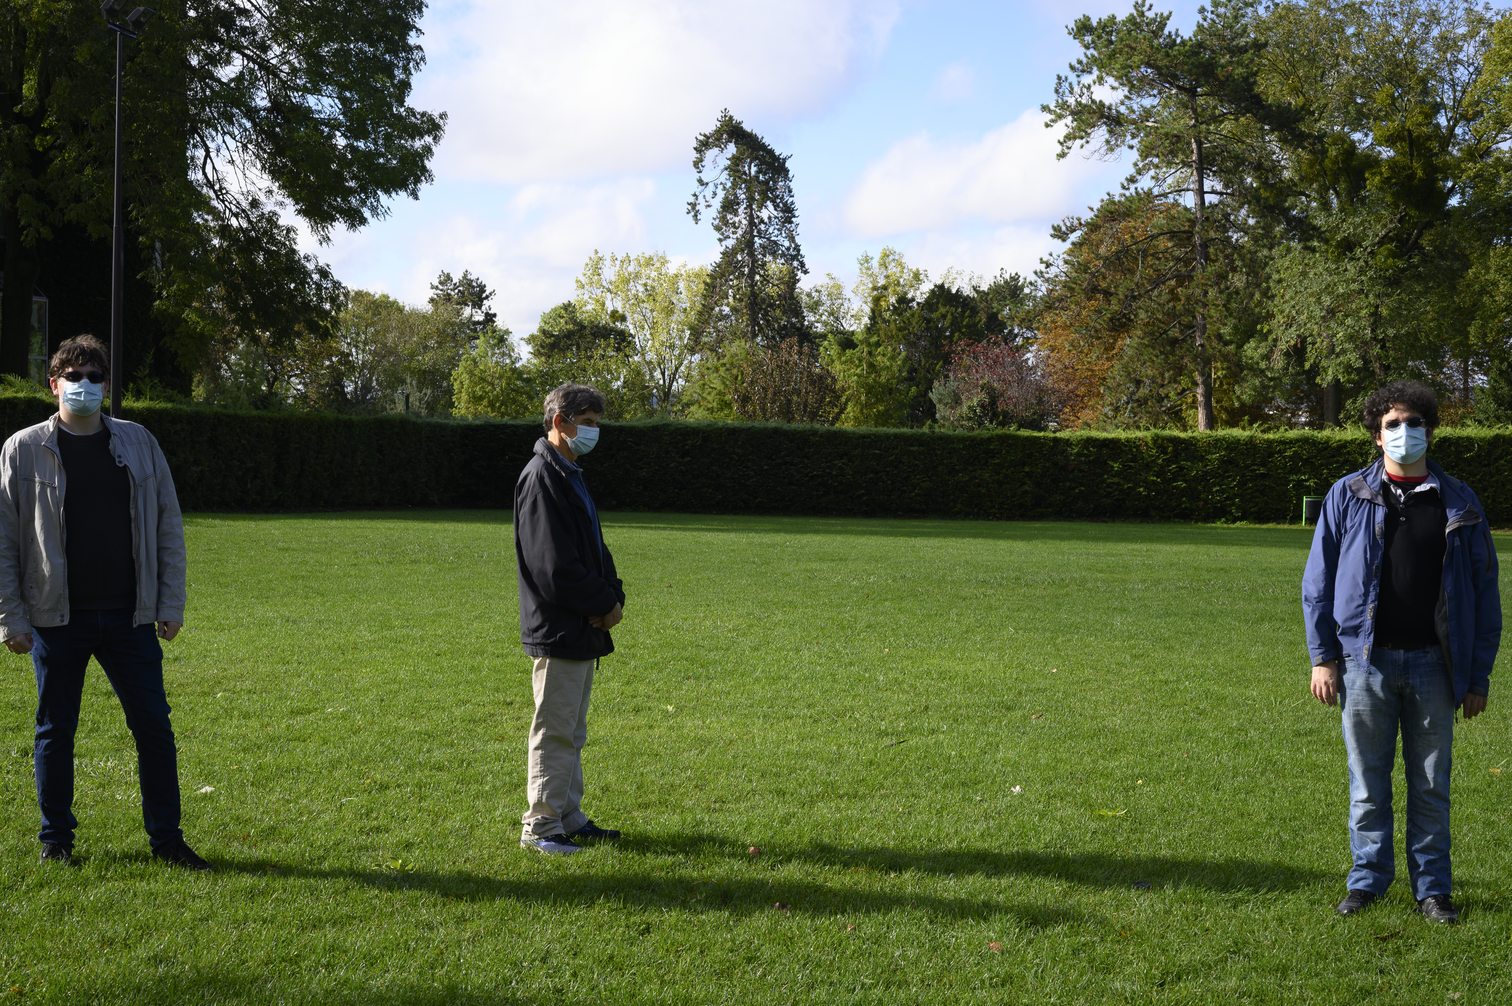
\includegraphics[width=.29\linewidth]{../assets/1512x1006/garden_fg_1.png}}  &
    \fbox{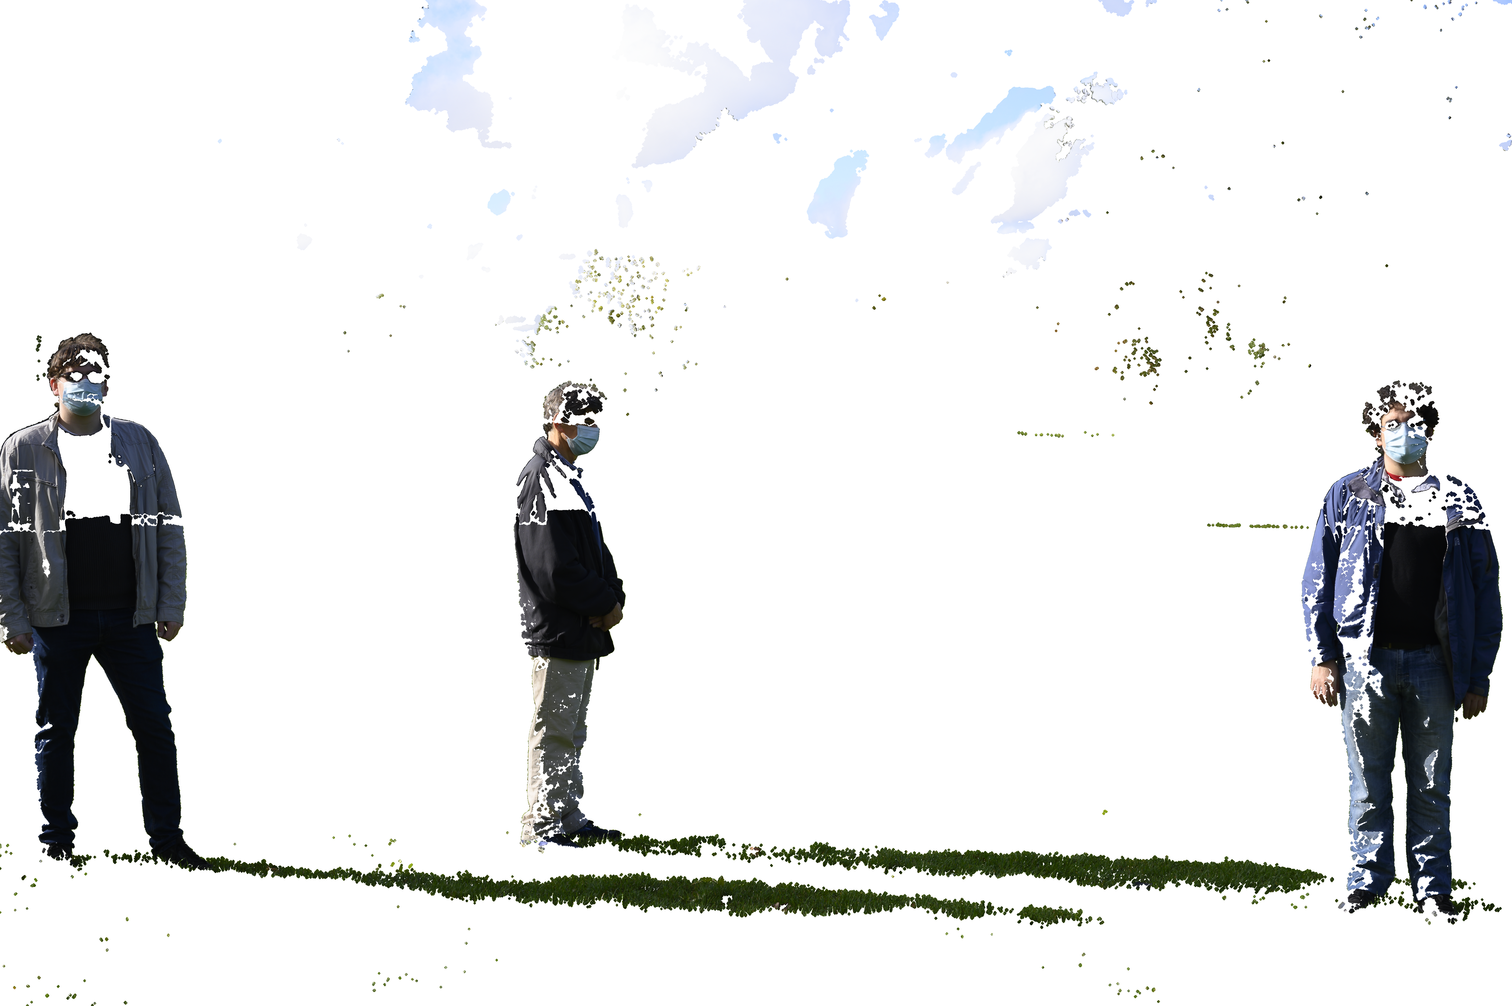
\includegraphics[width=.29\linewidth]{../assets/1512x1006/results_sig1_win5/garden/result_detected_garden_fg_1.png}} \\[5pt]
    \fbox{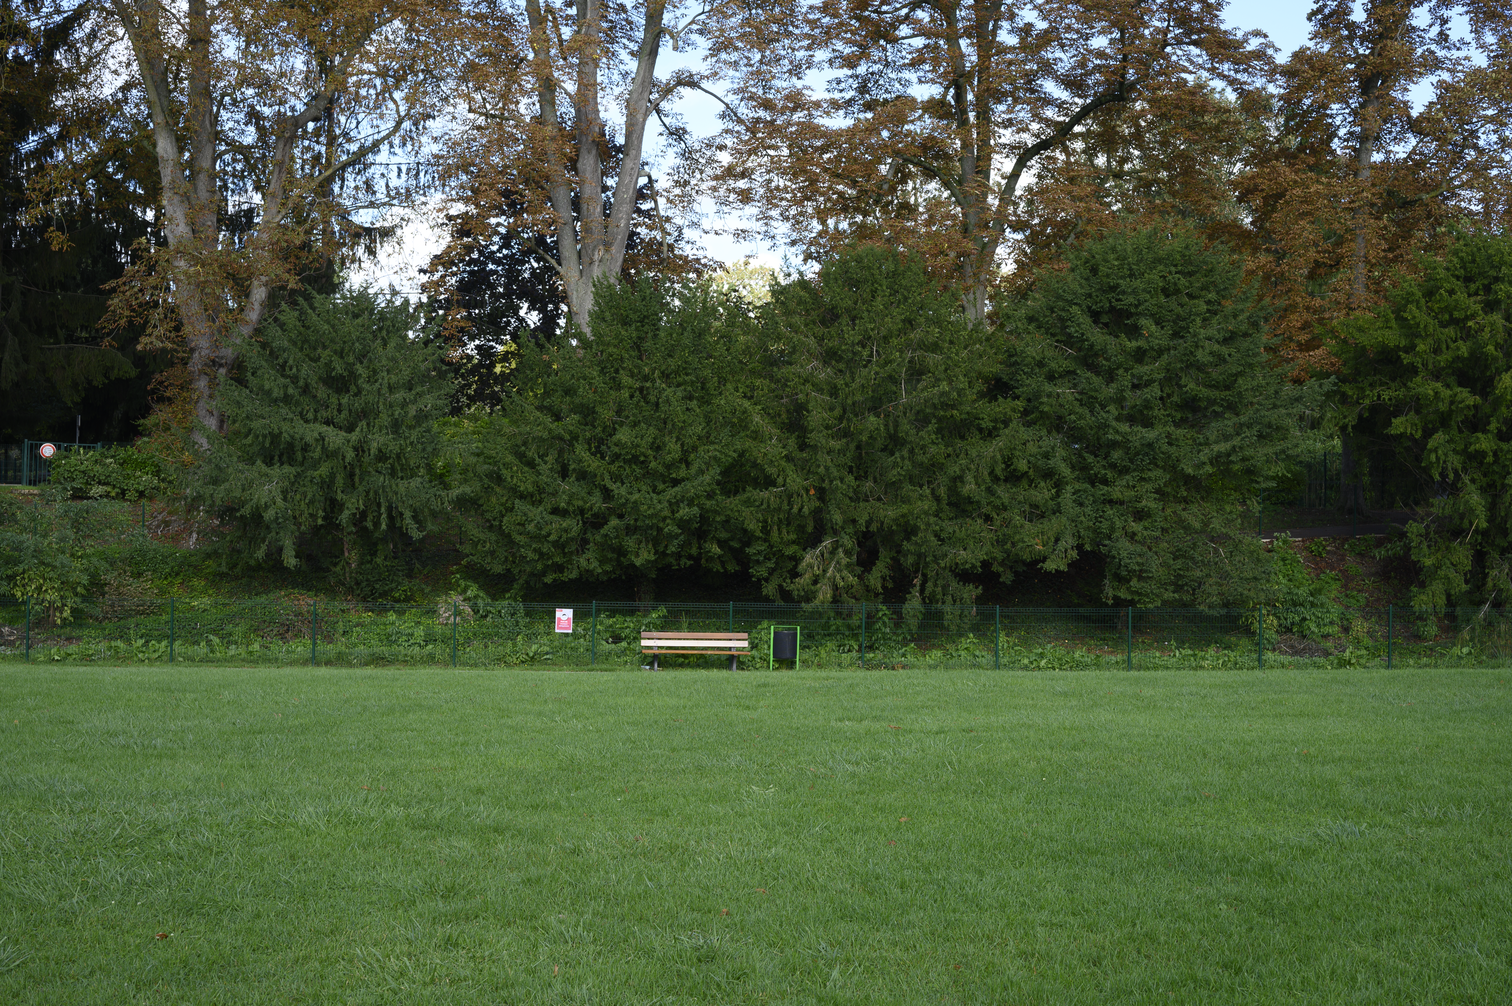
\includegraphics[width=.29\linewidth]{../assets/1512x1006/pathway_bg.png}}   &
    \fbox{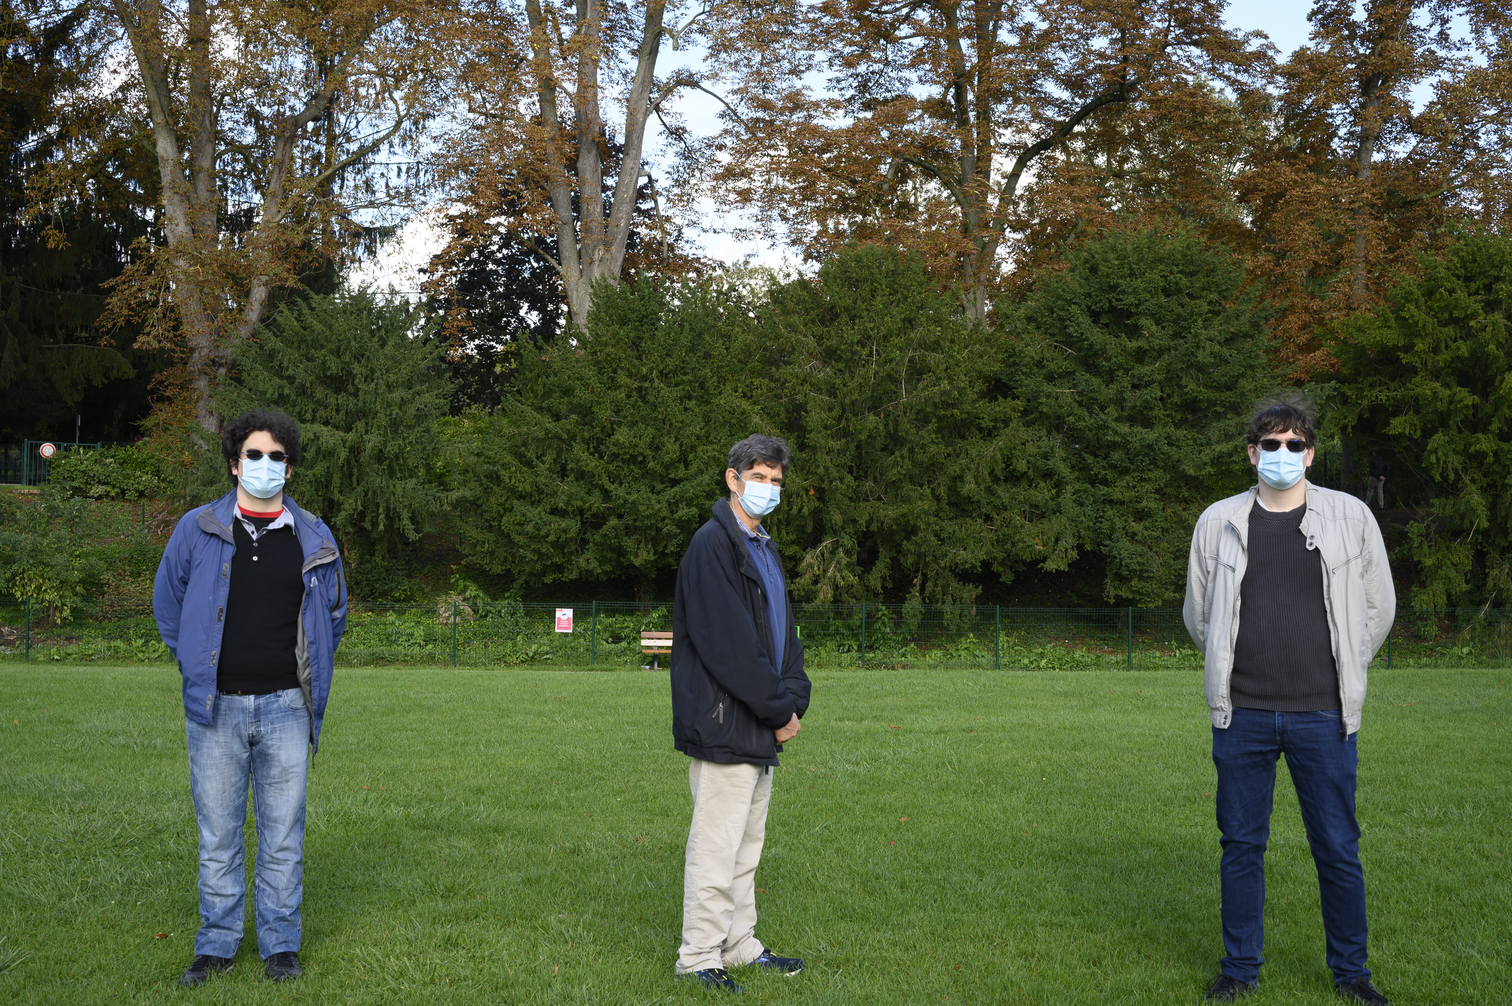
\includegraphics[width=.29\linewidth]{../assets/1512x1006/pathway_fg_1.png}} &
    \fbox{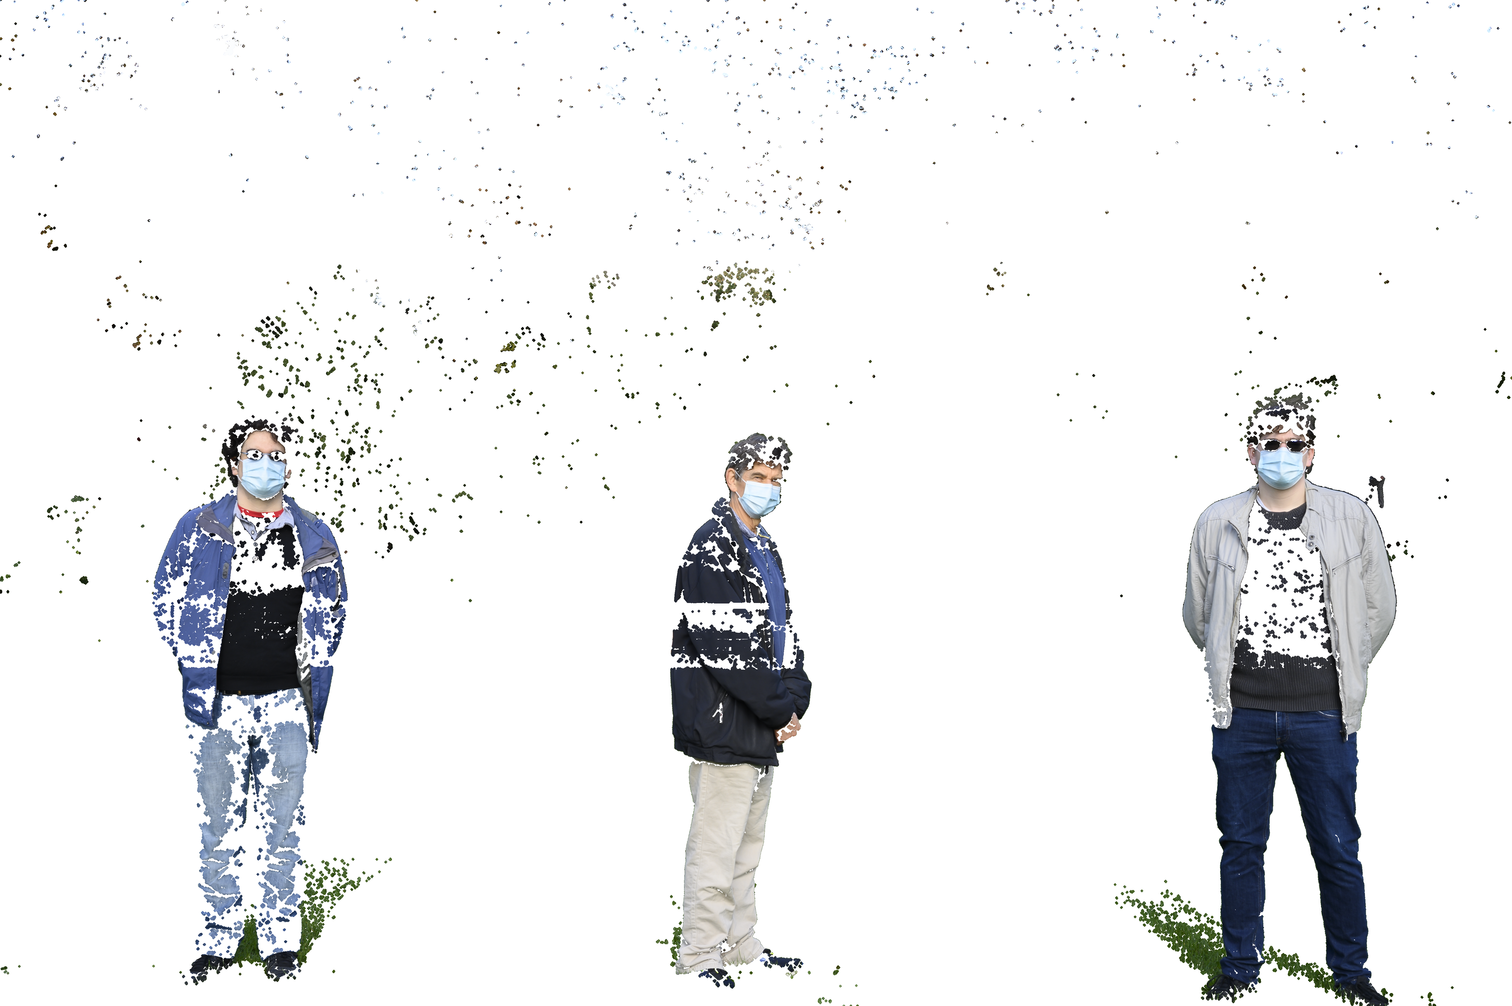
\includegraphics[width=.29\linewidth]{../assets/1512x1006/results_sig1_win5/pathway/result_detected_pathway_fg_1.png}}
  \end{tabular}

  \caption{Background detection: data set samples.}
  \label{fig:bg_sub.dataset_samples}
\end{figure}

We have run benchmarks on this set comparing multiple ways of achieving this result, both using Pylene and OpenCV as
well as varying the size and the shape of the structuring element window. The breakdown of these benchmarks are
presented in~\cref{fig:bg_sub.benchmarks}. In~\cref{table:views.perf}, we benchmark the computation time and the memory
usage~\footnote{Memory usage is computed with \emph{valgring/massif} as the difference between the memory peak of the
  run and the memory peak without any computation (just setup and image loading)}of these implementations (all
single-threaded) with an opening of disc of radius 32 on 10 MPix RGB images (the minimum of many runs is kept).

\begin{figure}[htbp]
  \centering
  \begin{tabular}{cccc}
    Result                                                                                                                       & Benchmark & Benchmark Pln only \\[5pt]
    \fbox{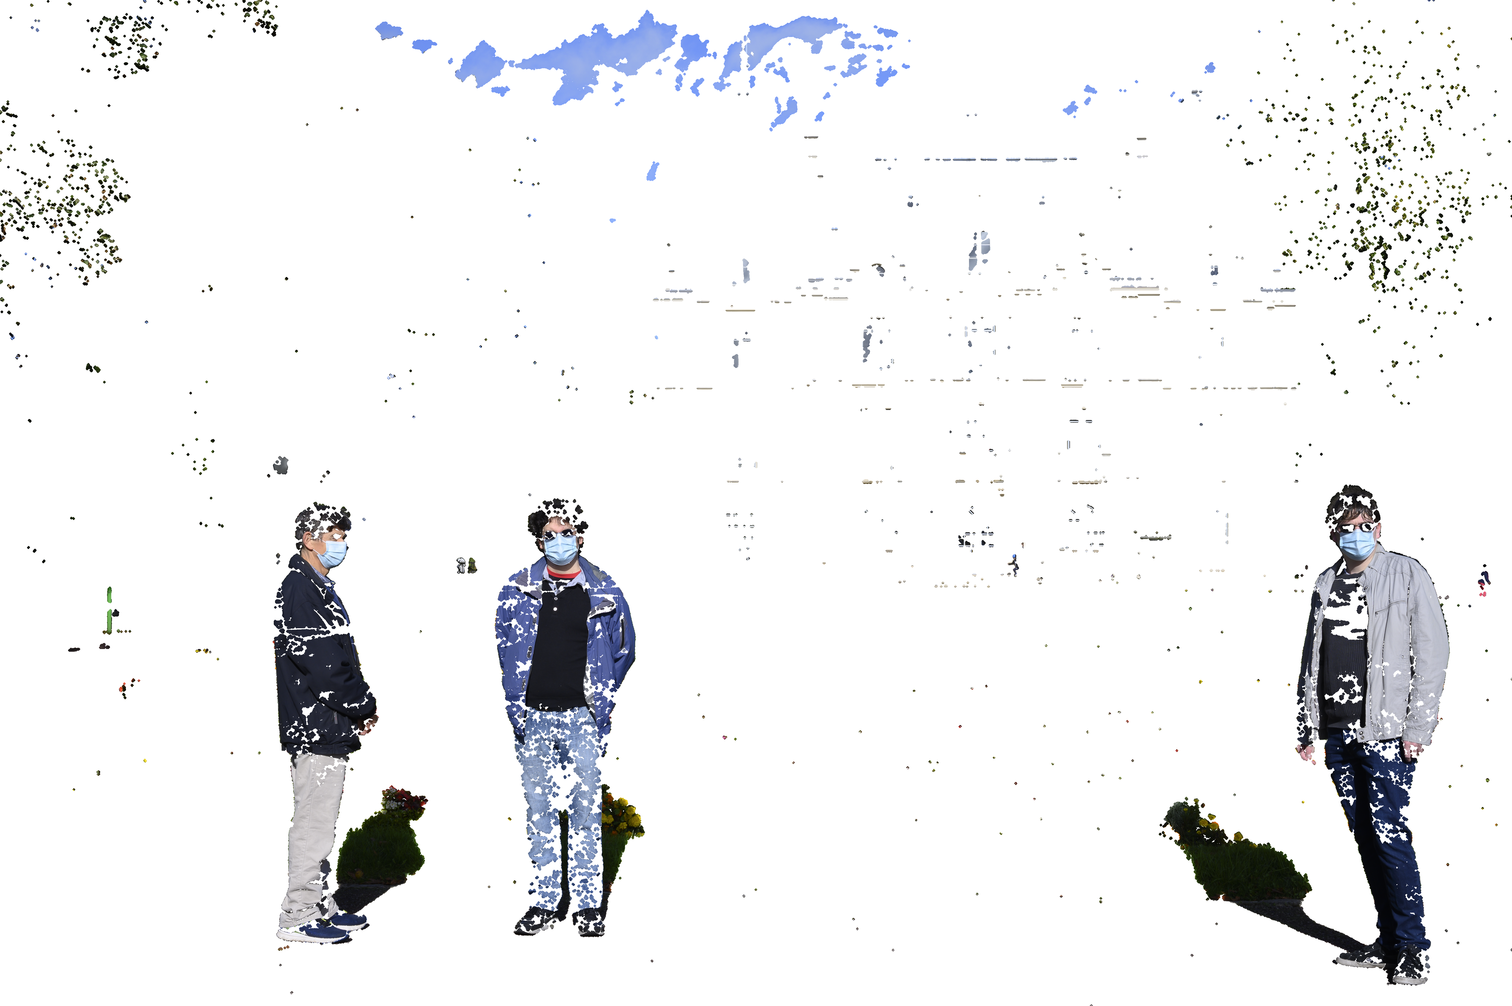
\includegraphics[width=.29\linewidth]{../assets/1512x1006/results_sig1_win5/castle/result_detected_castle_fg_1.png}}   &
    \fbox{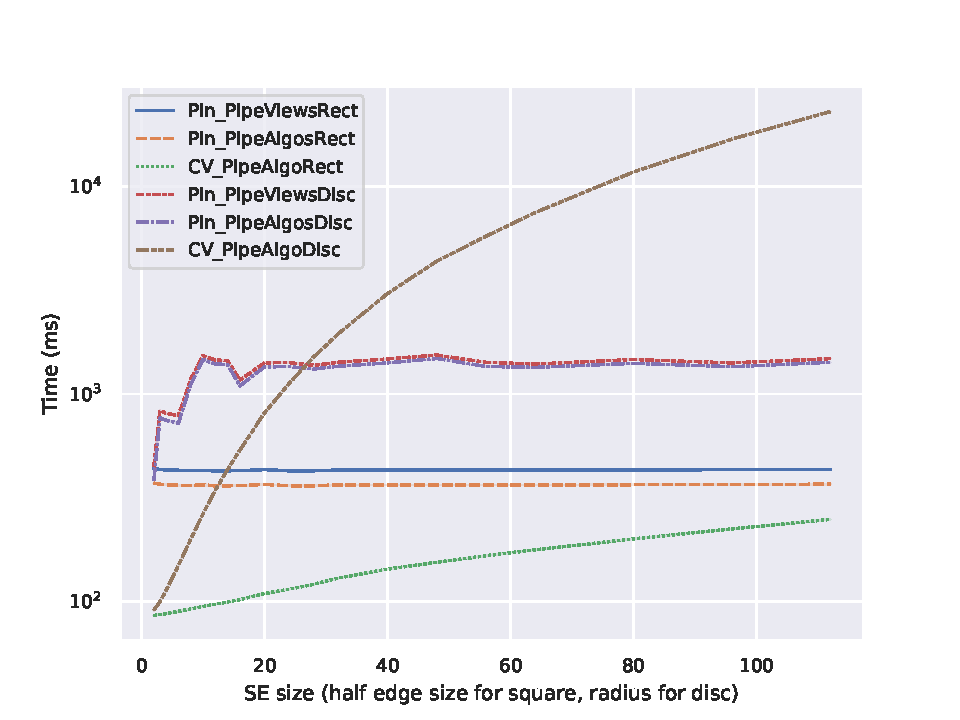
\includegraphics[width=.29\linewidth]{../figures/bench/PlnVsOpenCV_bg_sub_0}}                                          &
    \fbox{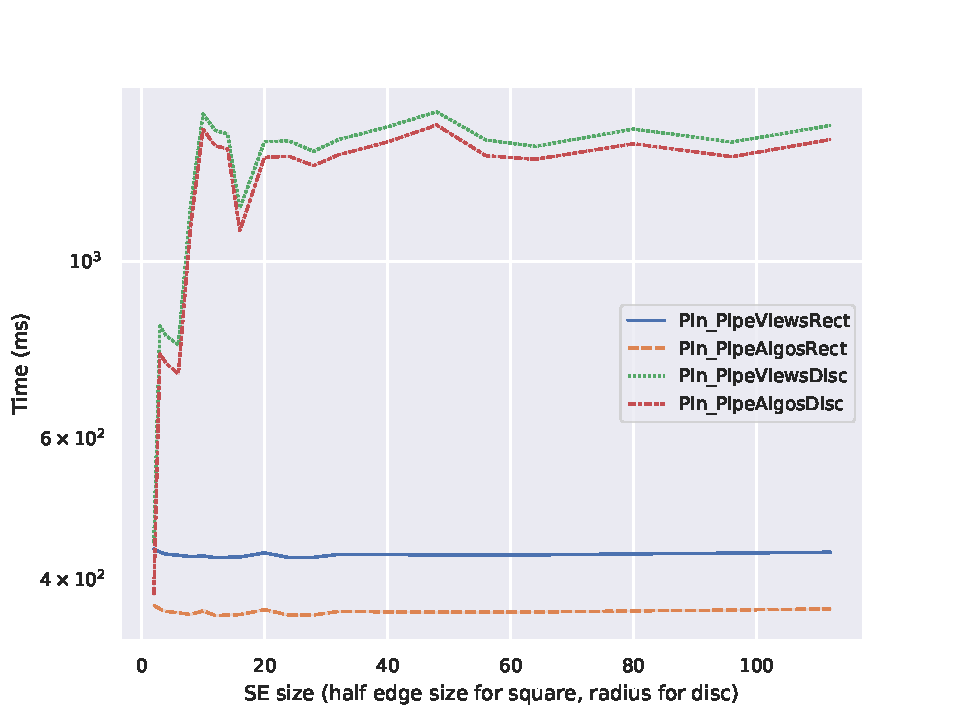
\includegraphics[width=.29\linewidth]{../figures/bench/PlnVsOpenCV_bg_sub_pln_0}}                                                                       \\[5pt]
    \fbox{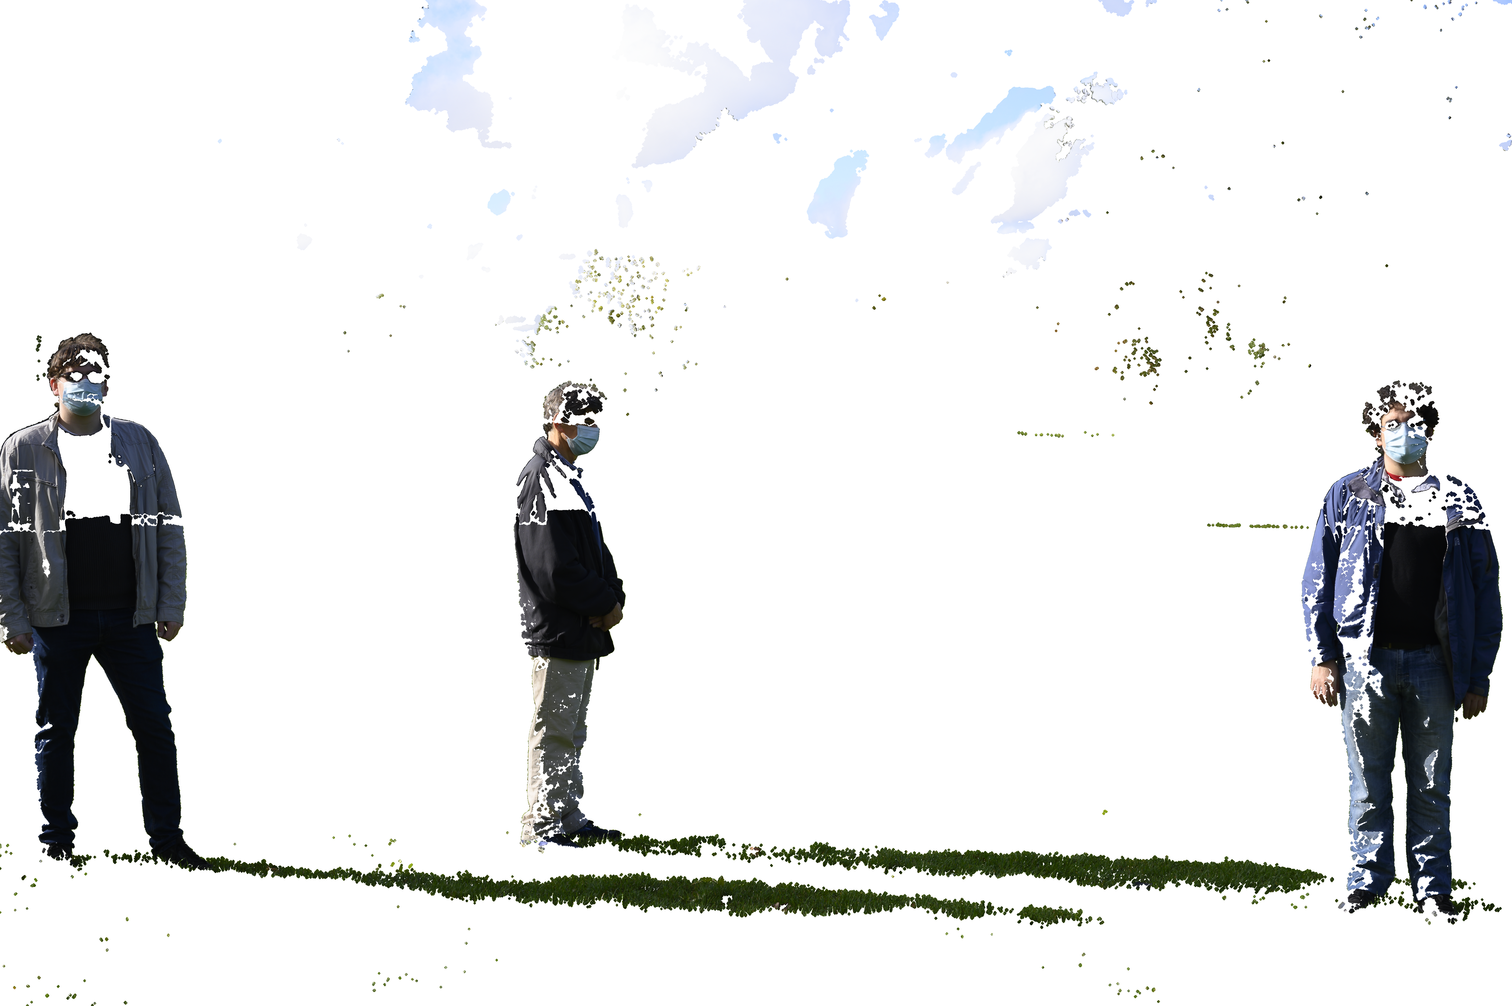
\includegraphics[width=.29\linewidth]{../assets/1512x1006/results_sig1_win5/garden/result_detected_garden_fg_1.png}}   &
    \fbox{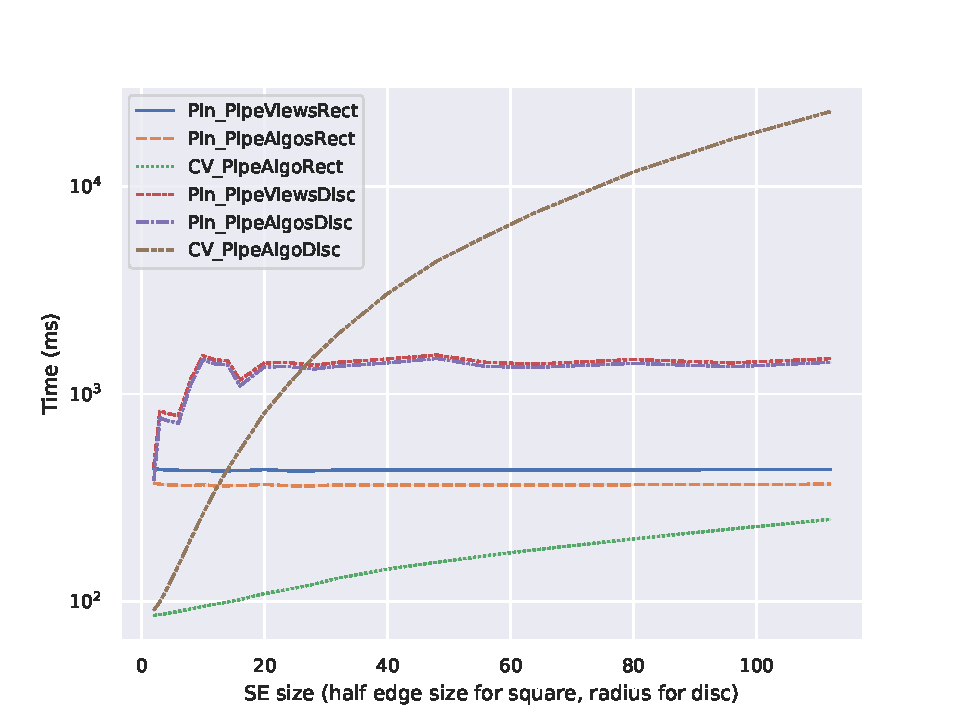
\includegraphics[width=.29\linewidth]{../figures/bench/PlnVsOpenCV_bg_sub_1}}                                          &
    \fbox{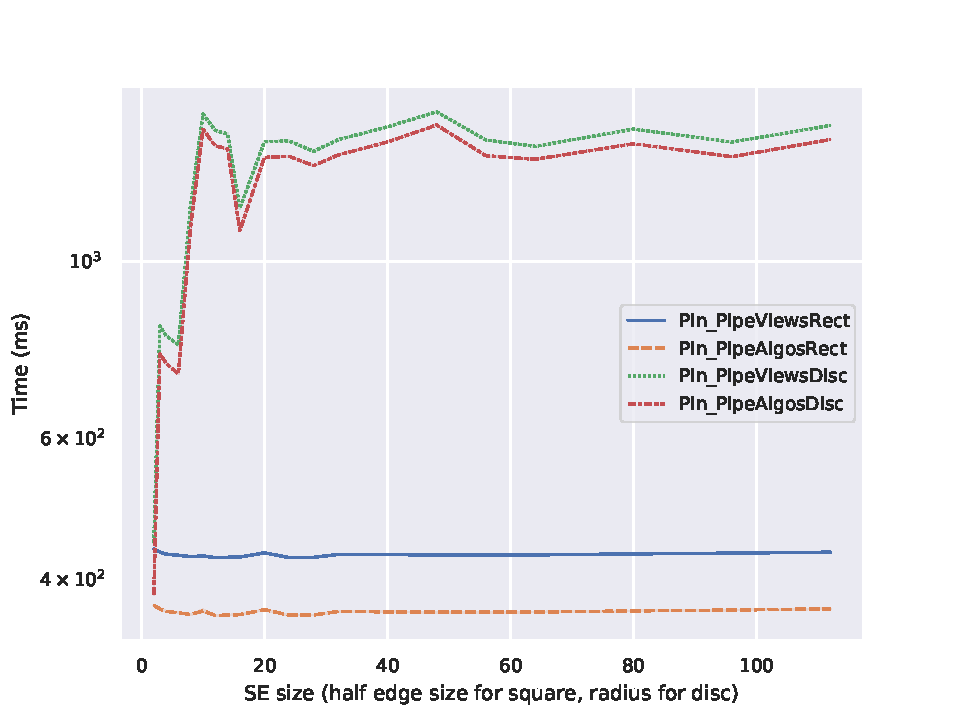
\includegraphics[width=.29\linewidth]{../figures/bench/PlnVsOpenCV_bg_sub_pln_1}}                                                                       \\[5pt]
    \fbox{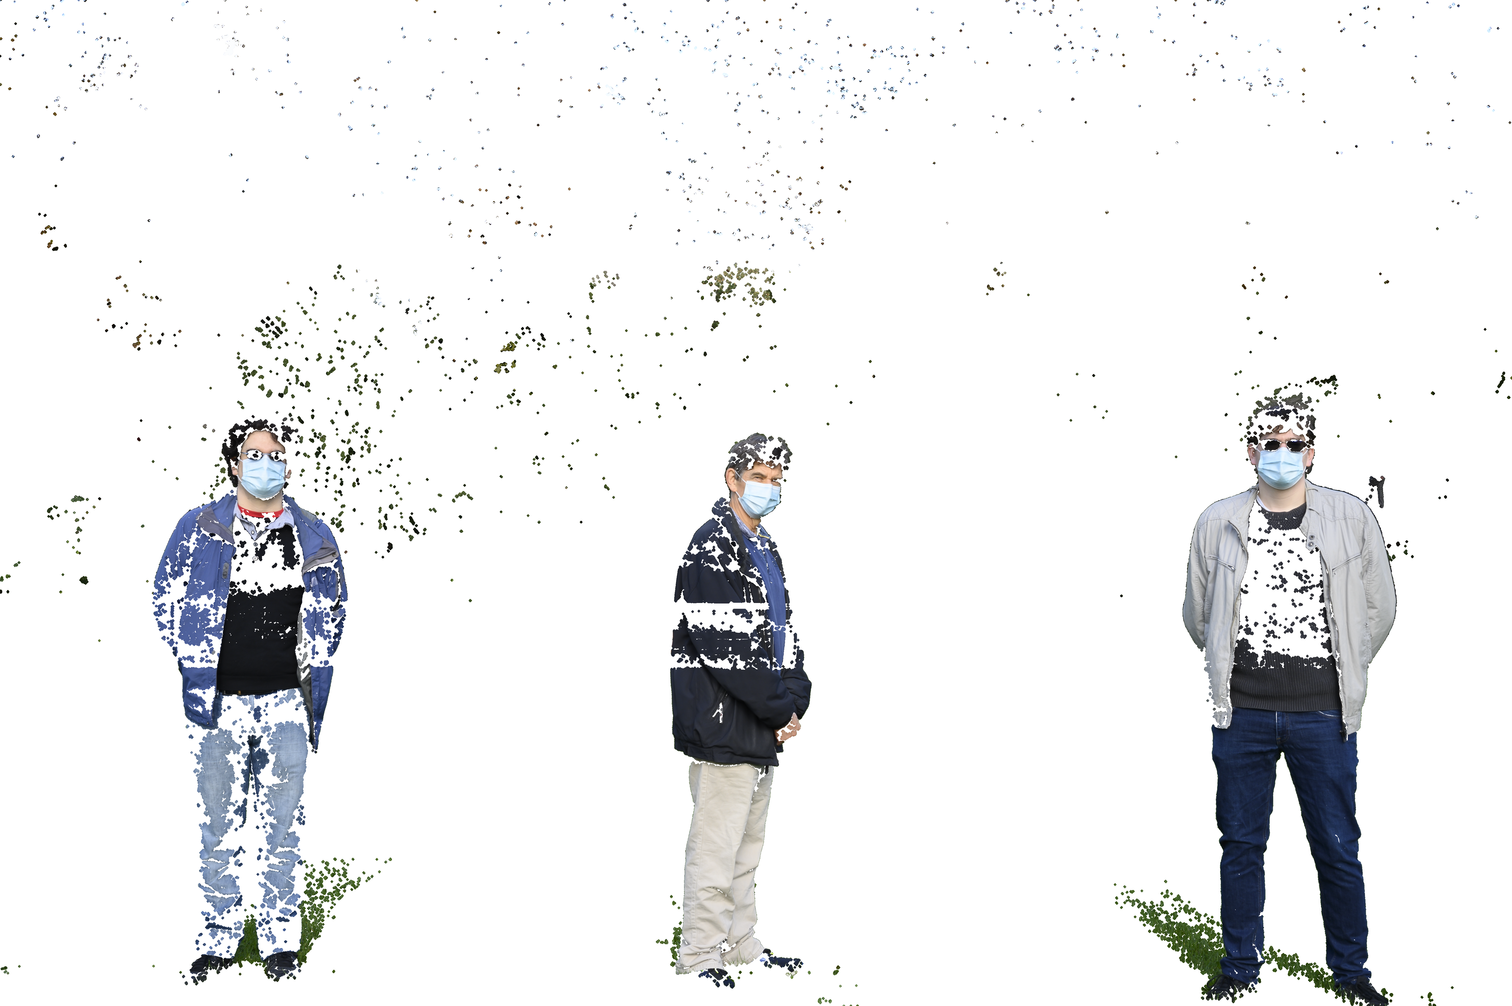
\includegraphics[width=.29\linewidth]{../assets/1512x1006/results_sig1_win5/pathway/result_detected_pathway_fg_1.png}} &
    \fbox{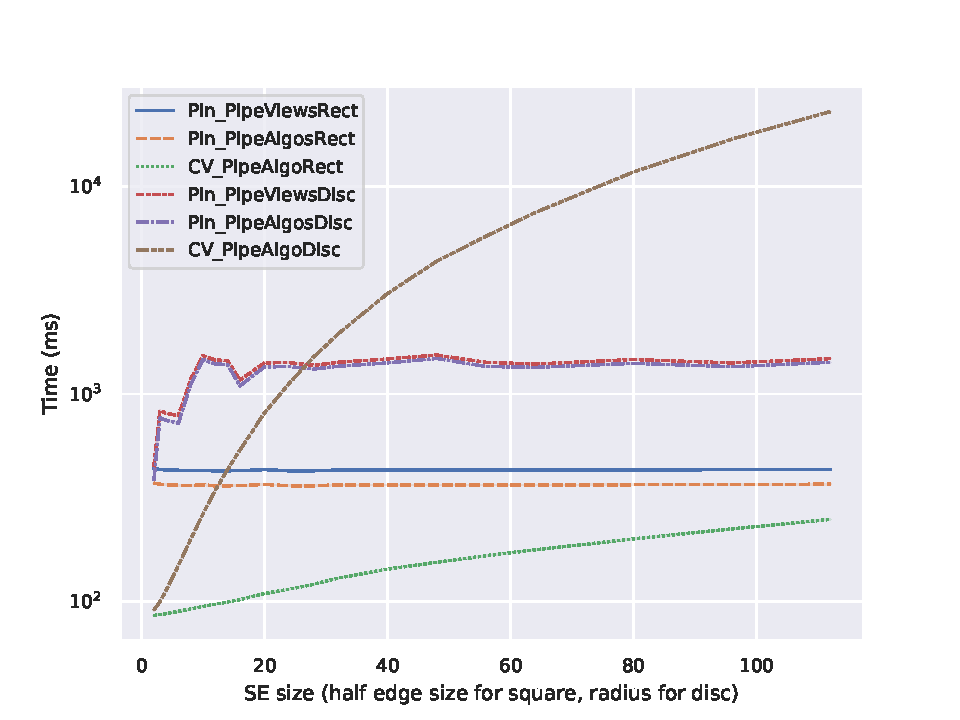
\includegraphics[width=.29\linewidth]{../figures/bench/PlnVsOpenCV_bg_sub_6}}                                          &
    \fbox{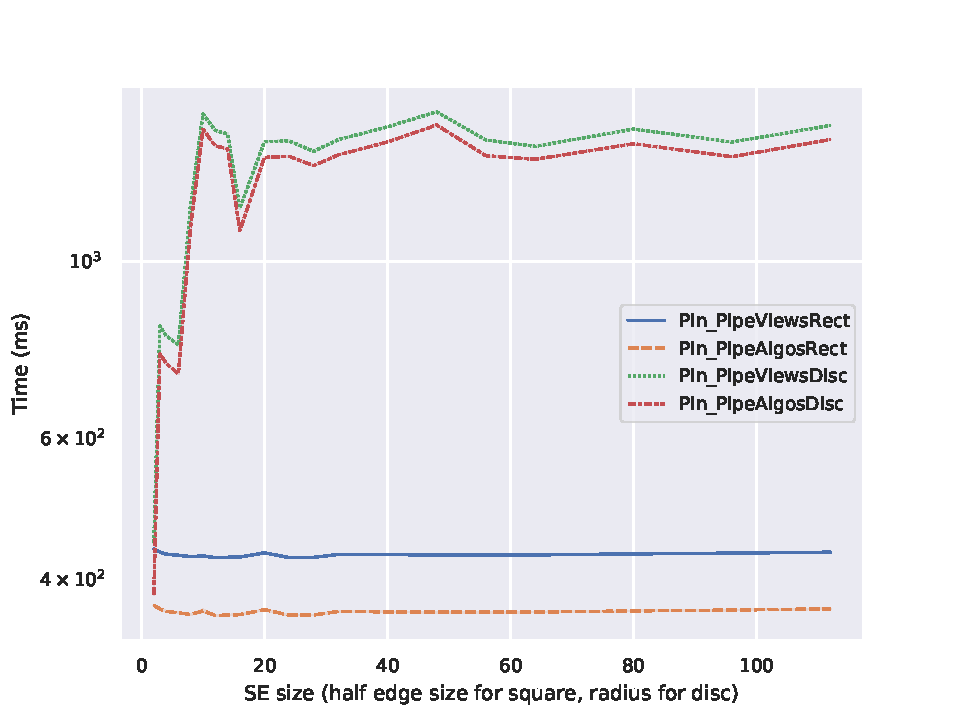
\includegraphics[width=.29\linewidth]{../figures/bench/PlnVsOpenCV_bg_sub_pln_6}}
  \end{tabular}

  \caption{Background detection: garden results.}
  \label{fig:bg_sub.benchmarks}
\end{figure}

\newcommand{\mystd}[1]{{\itshape(\(\pm\) #1)}}
\newcommand{\mydelta}[1]{{\itshape\bfseries #1\%}}

\begin{table}
  \centering
  \begin{tabular}{l|ccc}
    \toprule
    Framework          & Compute Time            & Memory usage & \(\Delta{}\)Memory usage \\ \midrule
    Pylene (w/o views) & \(2.11s\) \mystd{144ms} & 106 MB       & \mydelta{+0}             \\
    OpenCV             & \(2.41s\) \mystd{134ms} & 59 MB        & \mydelta{-44}            \\
    Pylene (views)     & \(2.13s\) \mystd{164ms} & 51 MB        & \mydelta{-52}            \\
    \bottomrule
  \end{tabular}
  \caption{Benchmarks of the pipeline \cref{fig:view.comp.sub_bg} on a dataset (12 images) of 10MPix images. Average
    computation time and memory usage of implementations with/without \emph{views} and with OpenCV as a baseline.}
  \label{table:views.perf}
  %\vspace{-1em}
\end{table}

The results should not be misunderstood. They do not say that OpenCV is faster or slower but shows that implementations
all have the same order of processing time (the algorithms used in our implementation are not the same as those used in
OpenCV for blur and dilation/erosion) so that the comparison makes sense. It allows us to validate experimentally the
advantages of views in pipelines. First, we have to be cautious about the real benefit in terms of processing time.
Here, most of the time is spent in algorithms that are not eligible for view transformation. Thus, depending on the
operations of the pipeline, views may not improve processing time. Nevertheless, using views does not degrade
performance neither (only 1\% in this experiment). It seems to show that using views does not introduce performance
penalties and may even be beneficial in lightweight pipelines as the one in~\cref{fig:view.pipeline}. On the memory
side, views reduce drastically the memory usage (also seen in~\cref{fig:legacy.vs.view}) which is beneficial when
developing applications which are memory constrained. From the developer standpoint, it requires only few changes in the
code as shown in~\cref{fig:view.comp.sub_bg.view_code} — the implementation of the algorithms remain the same — which is
a real advantage for software maintenance.


\section{Summary}

\paragraph{Views are composable.} One of the most important feature in a pipeline design (generally, in software
engineering) is \emph{object composition}. It enables composing simple blocks into complex ones. Those complex blocks
can then be managed as if they were still simple blocks. In~\cref{fig:view.pipeline}, we have 3 simple image operators
\emph{Image}~\(\rightarrow\)~\emph{Image} (the grayscale conversion, the sub-quantization and the dilation). As shown
in~\cref{fig:view.comp}, algorithm composition would consider these 3 simple operators as a single complex operator
\emph{Image}~\(\rightarrow\)~\emph{Image} that could then be used in another even more complex processing pipeline. Just
like algorithms, image views are composable, \eg a view of the view of an image is still an image.
In~\cref{fig:view.comp}, we compose the input image with a grayscale transform view and a sub-quantization view that
then feeds the dilation algorithm.

\paragraph{Views improve usability.} The code to compose images in~\cref{fig:view.comp} is almost as simple as:

\begin{minted}{c++}
auto input = imread(...);
auto A = transform(input, [](rgb16 x) -> float {
  return (x.r + x.g + x.b) / 3.f; }; );
auto MyComplexImage = transform(A, [](float x)
  -> uint8_t { return (x / 256 + .5f); }; );
\end{minted}

People familiar with functional programming may notice similarities with these languages where \emph{transform}
(\emph{map}) and \emph{filter} are sequence operators. Views use the functional paradigm and are created by functions
that take a function as argument: the operator or the predicate to apply for each pixel; we do not iterate by hand on
the image pixels.

\paragraph{Views improve re-usability.} The code snippets above are simple but not very re-usable. However, following
the functional programming paradigm, it is quite easy to define new views, because some image adaptors can be considered
as \emph{high-order functions} for which we can bind some parameters, as one would do with the curry
technique~\parencite{hanus.1995.curry}. In~\cref{fig:view.highorder}, we show how the primitive \emph{transform} can be
used to create a view summing two images and a view operator performing the grayscale conversion as well as the
sub-quantization which can be reused afterwards\footnote{These functions could have been written in a more generic way
  for more re-usability, but this is not the purpose here.}.

\begin{figure}
  \begin{minted}{c++}
auto operator+(Image A, Image B) {
  return transform(A, B, std::plus<>());
}
auto togray = [](Image A) { return transform(A, [](auto x)
  { return (x.r + x.g + x.b) / 3.f; };)
};
auto subquantize16to8b = [](Image A) { return transform(A,
  [](float x) { return uint8_t(x / 256 +.5f); });
};

auto input = imread(...);
auto MyComplexImage = subquantize16to8b(togray(A));
  \end{minted}

  \caption{Using high-order primitive views to create custom view operators.}
  \label{fig:view.highorder}
\end{figure}

\paragraph{Views for lazy computing.} Because the operation is recorded within the image view, this new image type
allows fundamental image types to be mixed with algorithms. In~\cref{fig:view.highorder}, the creation of views does not
involve any computation in itself but rather delays the computation until the expression \texttt{v(p)} is invoked.
Because views can be composed, the evaluation can be delayed quite far. Image adaptors are \emph{template
  expressions}~\parencite{veldhuizen.1995.expression, veldhuizen.2000.blitz} as they record the \emph{expression} used to
generate the image as a template parameter. A view actually represents an expression tree (\cref{fig:new.alphablend}).

\paragraph{Views for performance.} With a classical design, each operation of the pipeline is implemented on ``its
own''. Each operation requires memory to be allocated for the output image and also, each operation requires that the
image is fully traversed. This design is simple, flexible, composable, but is not memory efficient nor computation
efficient. With the lazy evaluation approach, the image is traversed only once (when the dilation is applied) which has
two benefits. First, there are no intermediate images which is very memory efficient. Second, traversing the image is
faster thanks to a better memory cache usage, and performs an optimal selective traversal. Indeed, in our example
(\cref{summary:fig:view.pipeline}), processing a RGB16 pixel from the dilation algorithm directly converts it in
grayscale, then sub-quantize it to 8-bits, and finally makes it available for the dilation algorithm. It acts \emph{as
  if} we were writing an optimal operator that would combine all these operations. This approach is somewhat related to
the kernel-fusing operations available in some HPC specifications~\parencite{openvx.2019} but views-fusion is optimized
by the C++ compiler only~\parencite{brown.2018.ranges}. The selective aspect intervenes when a region of interest is
selected at one point in the processing pipeline. Indeed, the entirety of the pipeline is then executed only on the
region of interest, even if this selection happens only at the very end of the processing pipeline.

\paragraph{Views for productivity.} All point-wise image processing algorithms can (and should) be rewritten intuitively
by using a one-liner view. The \emph{transform} views is the key enabling that point. This implies that there exist a
new abstraction level available to the practitioner when prototyping their algorithm. The time spent implementing
features is reduced, thus the feedback-loop time is reduced too. This naturally brings productivity gain to the
practitioner.
